\chapter{\titleof{c5}}
\label{chap:5}
\section{Introduction}
The success of deep neural networks to date depends strongly on the availability of labeled data. The more neural networks become deep and complex, the more it is crucial for them to be trained on massive amounts of training data. However, in many applications, labeled data is costly to obtain and task-specific training data is now a critical bottleneck. 

Usually it is much easier to obtain small quantities of high-quality labeled data and large quantities of unlabeled data. The problem of how to best integrate these two different sources of information during training is an active pursuit in the field of semi-supervised learning~\citep{chap:semi06}.
However, for a large class of tasks it is also easy to define one or more so-called ``weak annotators'', additional (albeit noisy) sources of \emph{weak supervision} based on heuristics or ``weaker'', biased classifiers trained on e.g.\ non-expert crowd-sourced data or data from different domains that are related. 
While easy and cheap to generate, it is not immediately clear if and how these additional weakly-labeled data can be used to train a stronger classifier for the task we care about.

More generally, in almost all practical applications, machine learning systems have to deal with data \emph{samples of variable quality}. For example, in a large dataset of images only a small fraction of samples may be labeled by experts and the rest may be crowd-sourced using e.g.\ Amazon Mechanical Turk~\citep{Veit:2017}. In addition, in some applications, labels are intentionally perturbed due to privacy issues~\citep{wainwright2012privacy,Papernot:2016, dehghani:2017:neuir}. 

Formally speaking, in our setup, we assume that we are given a large set of unlabeled data samples, a heuristic labeling function called the \emph{\wa}, and a small set of high-quality samples labeled by experts, called the \emph{strong dataset}, consisting of tuples of training samples $x_i$ and their true labels $y_i$, i.e. $\mathcal{D}_s=\{(x_i,y_i)\}$. We consider the latter to be observations from the true target function that we are trying to learn. 
We use the \wa to generate labels for the unlabeled samples. Generated labels are noisy due to the limited accuracy of the \wa. This gives us the \emph{weak dataset} consisting of tuples of training samples $x_i$ and their weak labels $\tilde{y}_i$, i.e. $\mathcal{D}_w=\{(x_i, \tilde{y}_i)\}$.  Note that we can generate a large amount of weak training data $\mathcal{D}_w$ at almost no cost using the \wa. In contrast, we have only a limited amount of observations from the true function, i.e. $|\mathcal{D}_s| \ll |\mathcal{D}_w|$. 

The simplest approach in this setup is to expand the strong training set, $\mathcal{D}_s$, by including the weakly-supervised samples, $\mathcal{D}_w$, which is in fact considering all samples are equally important. Alternatively, one may pretrain on the weak data and then fine-tune on observations from the true function or distribution (which we call strong data). Indeed, it has been shown that a small amount of expert-labeled data can be augmented in such a way by a large set of raw data, with labels coming from a heuristic function, to train a more accurate ranking model~\citep{Dehghani:2017:SIGIR, Severyn:2015:SIGIR}.
The downside is that such approaches are oblivious to the amount or source of noise in the labels. Simply speaking, they do not consider the cause of noise in the labels and only focus on the effect. 

In this chapter, we focus on this issue and try to address the following research question:
\resq{c5}

We argue that treating weakly-labeled samples uniformly (i.e.\ each weak sample contributes equally to the final classifier) ignores potentially valuable information of the label quality. 

Instead, we propose two different approaches that they directly model the inaccuracies introduced by the \wa, which can then be used to modulate the training process based on the fidelity (or quality) of each weak sample. 
% In other words, we control the extent to which we make use of this additional source of weak supervision: more for confidently-labeled weak samples close to the true observed data, and less for uncertain samples further away from the observed data. 


\subsection{Detailed Research Questions}
We break down our main research question in this chapter into two concrete research questions:
\begin{resqbox}
\begin{enumerate}
\item[\textbf{\resqname{c5.1}}] \emph{\resqcontnet{c5.1}}
\item[\textbf{\resqname{c5.2}}] \emph{\resqcontnet{c5.2}}
\end{enumerate}
\end{resqbox}
In the following sections, we will address these research questions, and support our ideas with experiments and analysis on different tasks.

\section{Learning to Learn from Weak Supervision, by Full Supervision}
\label{sec:meta_learning}
Using weak or noisy supervision is a straightforward approach to increase the size of the training data. This is usually done by pre-training the network on a large set of weakly labeled data and fine-tuning it with strong labels~\cite{Dehghani:2017:SIGIR,Severyn:2015:SIGIR}. 
However, these two independent stages do not leverage the full capacity of information from the small set of strong labels.  In particular, in the pre-training stage, we have to learn from labels of variable quality without any control over how these labels contribute to the learning process.

In this section, we address the first research question of this chapter:
\resq{c5.1}

We introduce a semi-supervised method that leverages a small amount of data with strong labels to improve the learning from a large amount of data with weak labels. This model, in fact, offers learning from \emph{Controlled Weak Supervision} and we refer to it by \emph{\cws} in the rest of this chapter.
%
\cws has three main components:
A \wa, which can be a heuristic model, a weak or biased classifier, or even a human via crowd-sourcing and it is employed to annotate a massive amount of unlabeled data, a \tnet, which uses a large set of weakly annotated instances by the \wa to learn the main task, and a \cnet, which is trained on a small set with strong labels to estimate confidence scores for instances annotated by the \wa. 

The confidence scores estimated by the \cnet define the magnitude of the weight updates applied to the \tnet during training. This way, the \cnet helps the \tnet to avoid the mistakes of her teacher, i.e., \wa, by down-weighting the weight updates from weak labels that do not look reliable according to \cnet.
%
\cws, in fact, employs teacher-student paradigm in which, the \tnet (student) and the \cnet (teacher) are trained jointly in a multi-task fashion and they share parameters of the representation learning layer to share their understanding of the data.

From a meta-learning perspective~\citep{Andrychowicz:2016,Finn2017:ICML,Ravi:2016}, the goal of the \cnet, as the meta-learner, trained jointly with the \tnet, as the learner, is to calibrate the learning rate of the \tnet for each instance in the batch. I.e., the weights $\pmb{w}$ of the \tnet $f_w$ at step $t+1$ are updated as follows:
\begin{equation}
\pmb{w}_{t+1} = \pmb{w}_t - \frac{\eta_t}{b}\sum_{i=1}^b c_{\theta}(x_i, \tilde{y}_i)  \nabla \mathcal{L}(f_{\pmb{w_t}}(x_i), \tilde{y_i})
%+ \nabla \mathcal{R}(\pmb{w_t})
\end{equation}
where $\eta_t$ is the global learning rate, $\mathcal{L}(\cdot)$ is the loss of predicting $\hat{y}=f_w(x_i)$ for an input $x_i$ when the label is $\tilde{y}$; $c_\theta(\cdot)$ is a scoring function learned by the \cnet taking input instance $x_i$ and its noisy label $\tilde{y}_i$. Thus, we can effectively control the contribution to the parameter updates for the \tnet from weakly labeled instances based on how reliable their labels are according to the \cnet (learned on a small supervised data).

Our setup requires running a \wa to label a large amount of unlabeled data, which is done at pre-processing time. For a large class of tasks, it is possible to use a simple heuristic, or implicit human feedback to generate weak labels. This set is then used to train the \tnet.  
In contrast, a small expert-labeled set is used to train the \cnet, which estimates how good the weak annotations are, i.e., controls the effect of weak labels on updating the parameters of the \tnet.

\cws allows learning different types of neural architectures and various tasks, where a meaningful \wa is available. 
Later in this chapter 

we study the performance of \cws by focusing on two applications: sentiment classification and document ranking. 

\subsection{Learning from Controlled Weak Supervision}
\label{sec:method}
In the following, we describe our recipe for semi-supervised learning of neural networks, in a scenario where along with a small human-labeled training set a large set of weakly labeled instances is leveraged.

% \subsection{General Architecture}
% \label{sec:generalarchitecture}
\begin{figure}[!t]%
    \makebox[\textwidth][c]{
    \centering
    \begin{subfigure}[t]{0.5\textwidth}
        \centering
        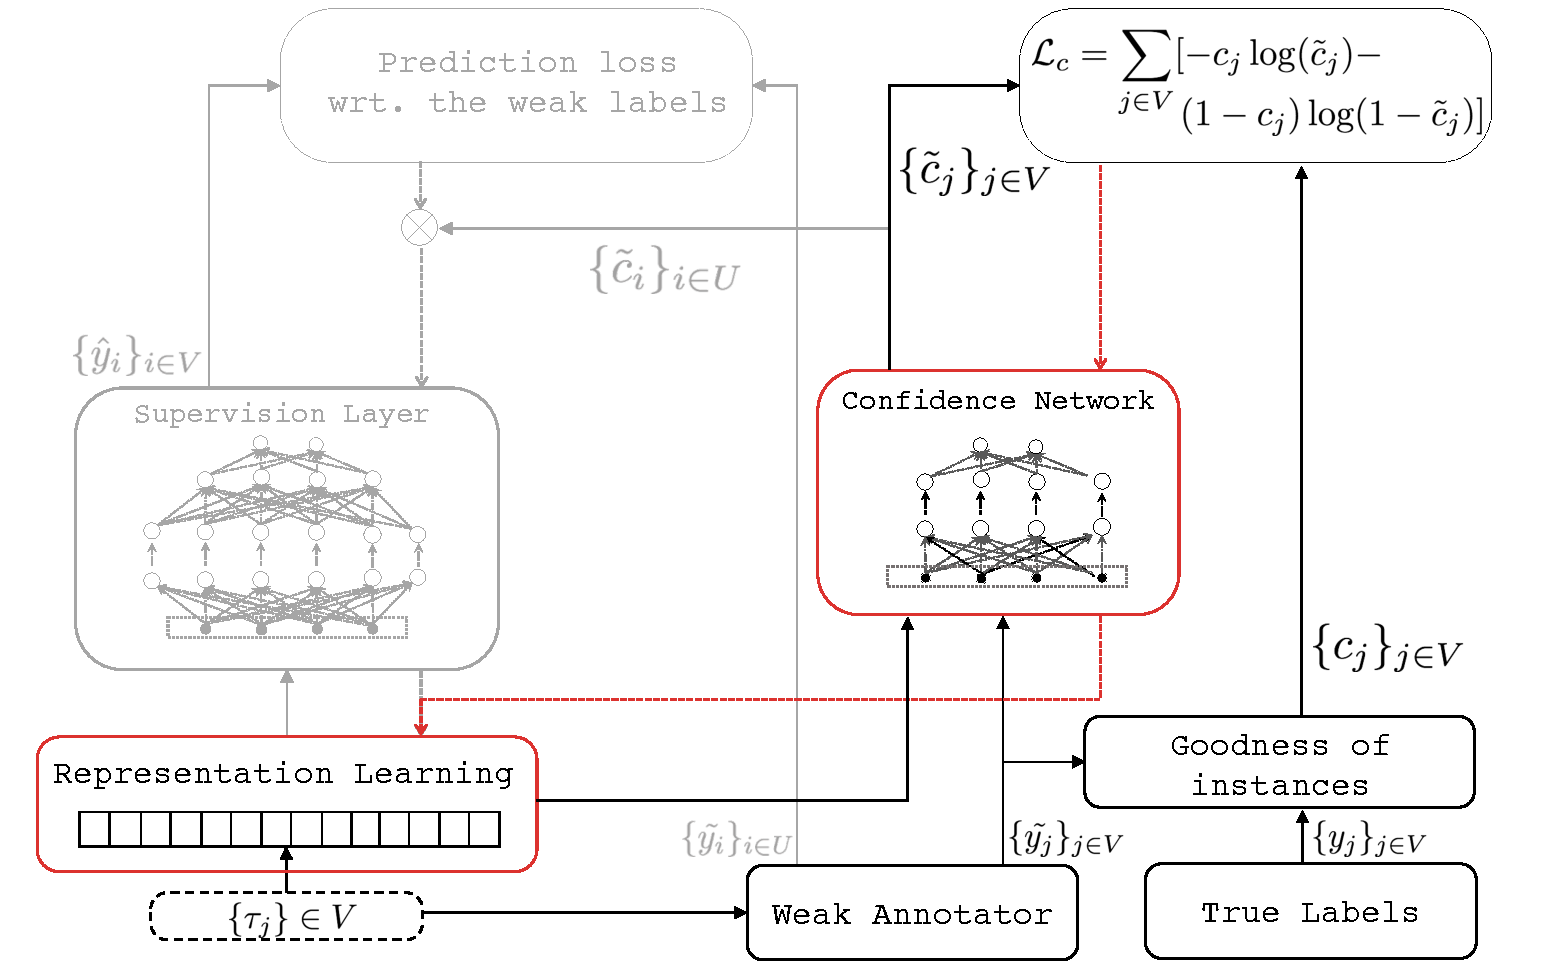
\includegraphics[width=\textwidth]{03-part-02/chapter-05/figs_and_tables/fig_cws_train_v.pdf}
        \caption{\label{fig:train_u}\footnotesize{Full Supervision Mode: Training on batches with strong labels.}}
    \end{subfigure}%
    ~
    \begin{subfigure}[t]{0.5\textwidth}
        \centering
        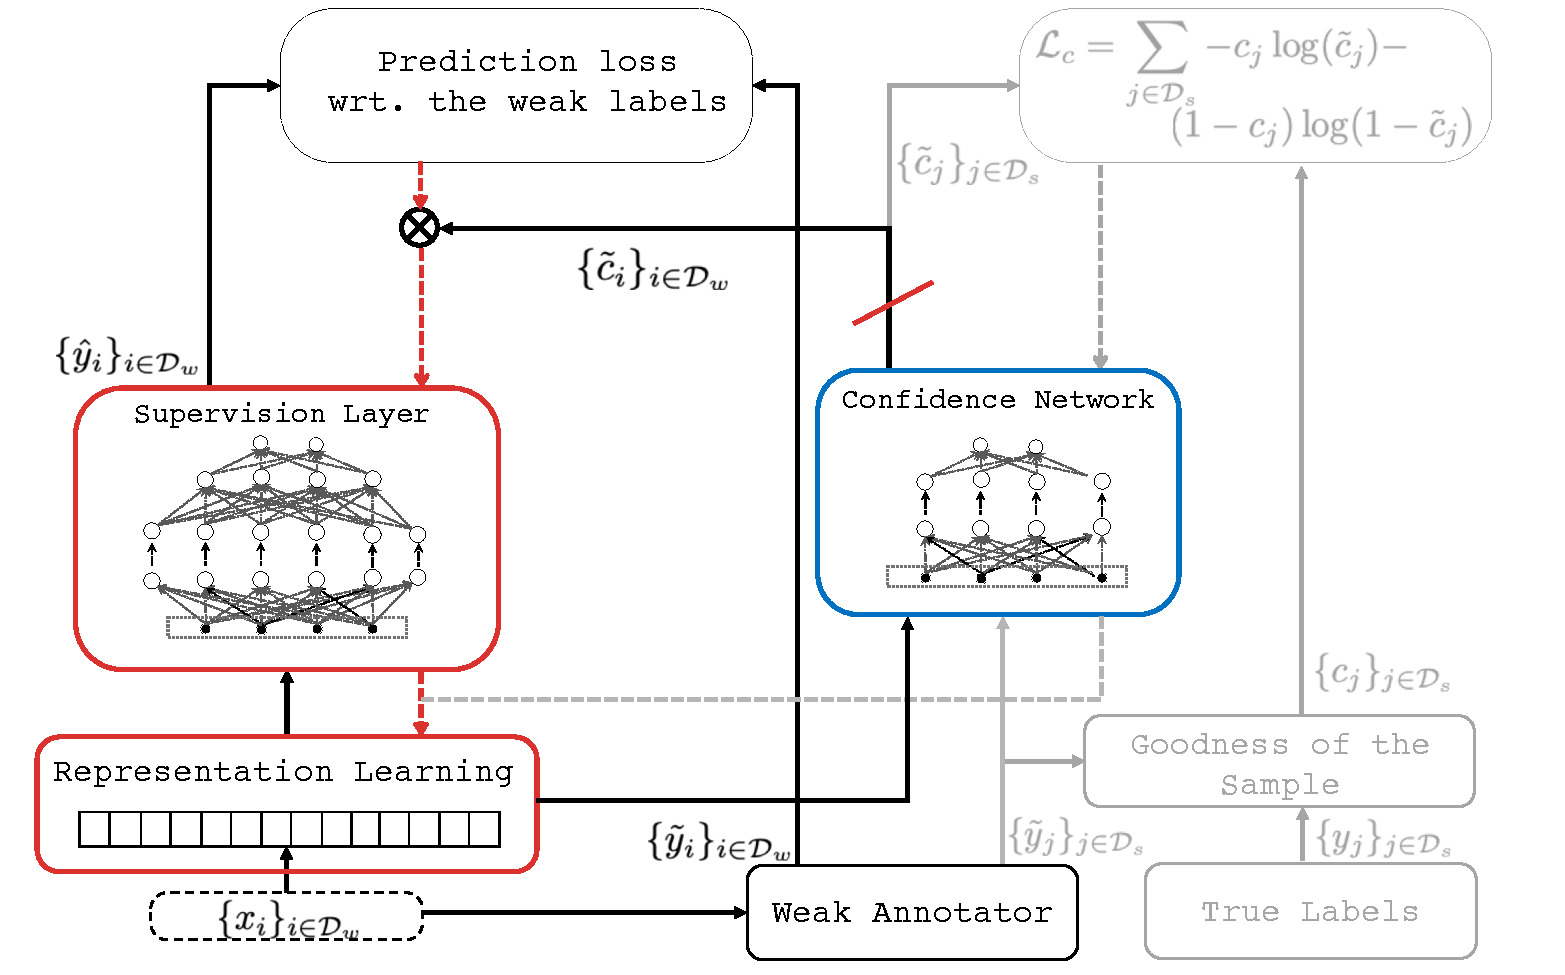
\includegraphics[width=\textwidth]{03-part-02/chapter-05/figs_and_tables/fig_cws_train_u.pdf}
        \caption{\label{fig:train_v}\footnotesize{Weak Supervision Mode: Training on batches with weak labels.}}
    \end{subfigure}%
    }
    \caption{Learning from controlled weak supervision: Our proposed multi-task network for learning a target task in a semi-supervised fashion, using a large amount of weakly labeled data and a small amount of data with strong labels.
    %
    Faded parts of the network are disabled during the training in the corresponding mode. Red-dotted arrows show gradient propagation. Parameters of the parts of the network in red frames get updated in the backward pass, while parameters of the network in blue frames are fixed during the training. (Best viewed in color.)}
    \label{fig:model_cws}
\end{figure}

In our proposed model we train a multi-task neural network that jointly learns the confidence score of weakly labeled instances and the main task using controlled supervised signals.
%
The high-level representation of the model is shown in Figure~\ref{fig:model_cws}: it comprises a \wa and two neural networks: the \cnet and the \tnet. 

The goal of the \wa is to \emph{provide weak labels} $\tilde{y}_i$ for all the instances $x_i \in U \cup V$. We have this assumption that $\tilde{y}_i$ provided by the \wa are imperfect estimates of strong labels $y_i$, where $y_i$ are available for set $\mathcal{D}_s$, but not for set $\mathcal{D}_w$.

The goal of the \cnet is to \emph{estimate the confidence score} $\tilde{c}_j$ of training instances. It is learned on examples from the training set $\mathcal{D}_s$, i.e a set of input $x_j$ and its strong label $y_j$ as well its weak label,  $\tilde{y}_j$,  that is annotated by the \wa.
The score $\tilde{c}_j$ is then used to control the effect of weakly labeled instances on updating the parameters of the \tnet in the backward pass of backpropagation.

The \tnet is in charge of \emph{handling the main task} we want to learn, or in other words, approximating the underlying function that predicts the correct labels. 
Given the data instance, $x_i$ and its weak label $\tilde{y}_i$ from the training set $\mathcal{D}_w$, the \tnet aims to predict the label $\hat{y}_i$. 
The \tnet parameter updates are based on noisy labels assigned by the \wa, but the magnitude of the gradient update is based on the output of the \cnet. 

Both networks are trained in a multi-task fashion alternating between the \emph{full supervision} and the \emph{weak supervision} mode.  
In the \emph{full supervision} mode, the parameters of the \cnet get updated using instances from training set $\mathcal{D}_s$.  
As depicted in Figure~\ref{fig:train_v}, each training instance is passed through the representation layer mapping inputs to vectors. These vectors are concatenated with their corresponding weak labels $\tilde{y}_j$ generated by the \wa.
The \cnet, which is a fully connected feedforward network with sigmoid as the output layer, estimates $\tilde{c}_j$ that is the probability of taking data instance $j$ into account for training the \tnet.

In the \emph{weak supervision} mode, the parameters of the \tnet are updated using the training set $\mathcal{D}_w$.
As shown in Figure~\ref{fig:train_u}, each training instance is passed through the same representation learning layer and is then processed by the supervision layer which is a part of the \tnet predicting the label for the main task. 
%
We also pass the learned representation of each training instance along with its corresponding label generated by the \wa to the \cnet to estimate the \emph{confidence score} of the training instance, i.e., $\tilde{c}_i$. 
The confidence score is computed for each instance from the training set $\mathcal{D}_w$. These confidence scores are used to weight the gradient updating \tnet parameters or in other words the step size during back-propagation. 

It is noteworthy that the representation layer is shared between both networks, so besides the regularization effect of layer sharing which leads to better generalization, sharing this layer lays the ground for the \cnet to benefit from the largeness of the set $\mathcal{D}_w$ and the \tnet to utilize the quality of set $\mathcal{D}_s$. 

\subsection{Training the Learner and the Meta-Learner}
\label{sec:modeltraining}
Here, we explain how we train \cws in which we jointly update the parameters of \tnet, the learner and the \cnet, the meta-learner. 
Our optimization objective is composed of two terms: (1) the \cnet loss $\mathcal{L}_c$, which captures the quality of the output from the \cnet and (2) the \tnet loss $\mathcal{L}_t$, which expresses the quality for the main task. 

Both networks are trained by alternating between the \emph{weak supervision} and the \emph{full supervision} mode.
%
In the \emph{full supervision} mode, the parameters of the \cnet are updated using training instance drawn from training set $\mathcal{D}_s$. We use cross-entropy loss function for the \cnet to capture the difference between the predicted confidence score of instance $j$, i.e., $\tilde{c}_j$ and the target score $c_j$:
\begin{equation}
% \nonumber
\mathcal{L}_c = \sum_{j\in V} -  c_j \log(\tilde{c}_j) - (1-c_j) \log(1-\tilde{c}_j),
\end{equation}
%given that $c_j$ is not a probability I'm wondering if we can call this loss a cross-entropy --- it only makes sense if $c_j$ is a probability of binary event. Possibly, it's common to use in IR, but i've never seen it used like this on real-valued scores.} 
The target score $c_j$ indicates how similar the strong and the weak labels are, and it is calculated with respect to the main task. 

In the \emph{weak supervision} mode, the parameters of the \tnet are updated using training instances from $\mathcal{D}_w$. We use a weighted loss function, $\mathcal{L}_t$, to capture the difference between the predicted label $\hat{y}_i$ by the \tnet and target label $\tilde{y}_i$:
\begin{equation}
% \nonumber
\mathcal{L}_t = \sum_{i\in U} \tilde{c}_i \mathcal{L}_i,
\end{equation}
where $\mathcal{L}_i$ is the task-specific loss on training instance $i$ and $\tilde{c}_i$ is the confidence score of the weakly annotated instance $i$, estimated by the \cnet.
Note that $\tilde{c}_i$ is treated as a constant during the weak supervision mode and there is no gradient propagation to the \cnet in the backward pass (as depicted in Figure~\ref{fig:train_u}). 

We minimize two loss functions jointly by randomly alternating between full and weak supervision modes (for example, using a 1:10 ratio).
During training and based on the chosen supervision mode, we sample a batch of training instances from $\mathcal{D}_s$ with replacement or from $\mathcal{D}_w$ without replacement (since $\mathcal{D}_w$ can be very large). Since in our setups usually $|\mathcal{D}_w| >> \mathcal{D}_s|$, the training process oversamples the instance from $\mathcal{D}_s$. 

The key point here is that the ``main task'' and ``confidence scoring'' task are always defined to be close tasks and sharing representation will benefit the confidence network as an implicit data augmentation to compensate the small amount of data with strong labels.
Besides, we noticed that updating the representation layer with respect to the loss of the other network acts as a regularization for each of these networks and helps generalization for both target and confidence network since we try to capture all tasks (which are related tasks) and less chance for overfitting.

% We also investigated other possible setups or training scenarios. For instance, we tried updating the parameters of the supervision layer of the \tnet using also data with strong labels. Or instead of using alternating sampling, we tried training the \tnet using controlled weak supervision signals after the \cnet is fully trained.
% As shown in the experiments the architecture and training strategy described above provide the best performance.
\newcommand{\tfunc}{T} %function name for the teacher
\section{\fwlfull}
\label{sec:fidelity_weighted_learning}

In this section, we address the second research question of this chapter:
\resq{c5.2}

We introduce \fwlfull (\fwl), a Bayesian semi-supervised approach that leverages a small amount of data with strong labels to generate a larger training set with \emph{confidence-weighted weakly-labeled samples}, which can then be used to modulate the fine-tuning process based on the fidelity (or quality) of each weak sample. By directly modeling the inaccuracies introduced by the \wa in this way, we can control the extent to which we make use of this additional source of weak supervision: more for confidently-labeled weak samples close to the true observed data, and less for uncertain samples further away from the observed data. We use a non-parametric kernel-based method to measure the closeness.

We propose a setting consisting of two main modules. One is called the \std and is in charge of learning a suitable data representation and performing the main prediction task (similar to the \tnet in Section~\ref{sec:meta_learning}), the other is the \tch which modulates the learning process by modeling the inaccuracies in the labels. 

\begin{figure}[!t]%
    \makebox[\textwidth][c]{
    \centering
    \begin{subfigure}[t]{0.325\textwidth}
        \centering
        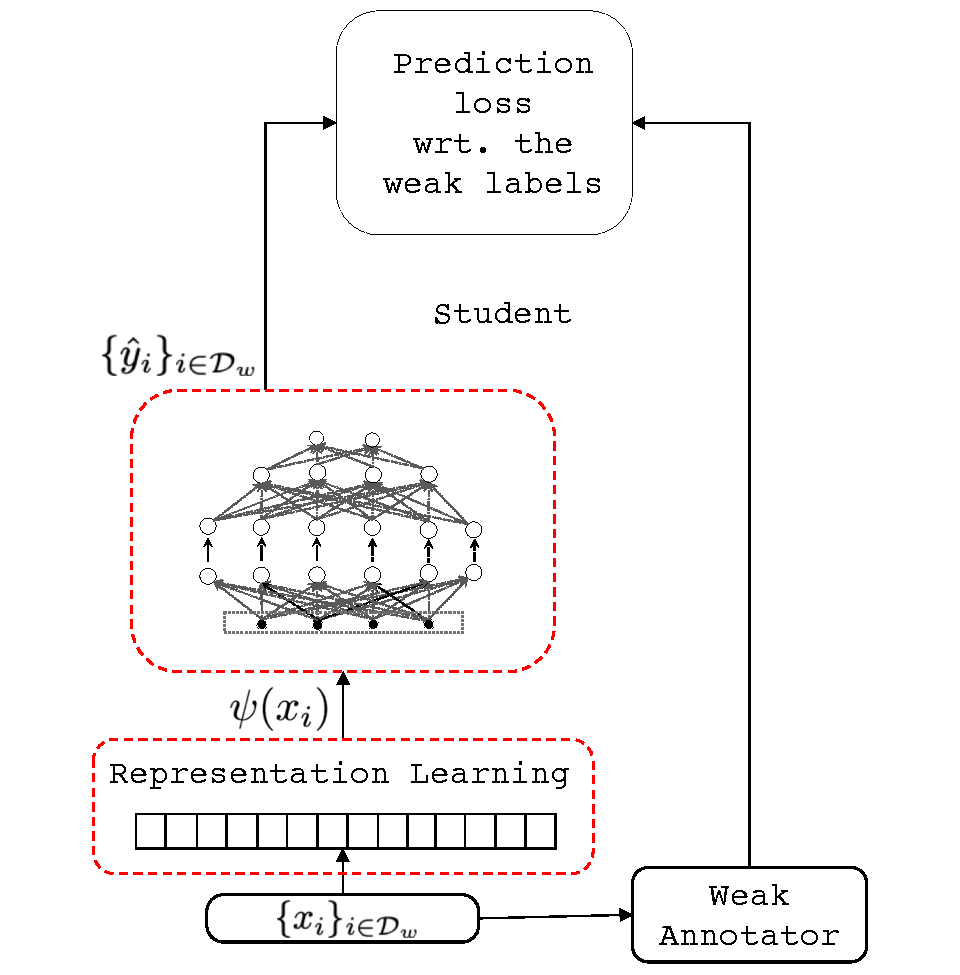
\includegraphics[width=\textwidth]{03-part-02/chapter-05/figs_and_tables/fig_fwl_step_1.pdf}
        \caption{\label{fig:step1}Step 1}
    \end{subfigure}%
    ~
    \begin{subfigure}[t]{0.25\textwidth}
        \centering
        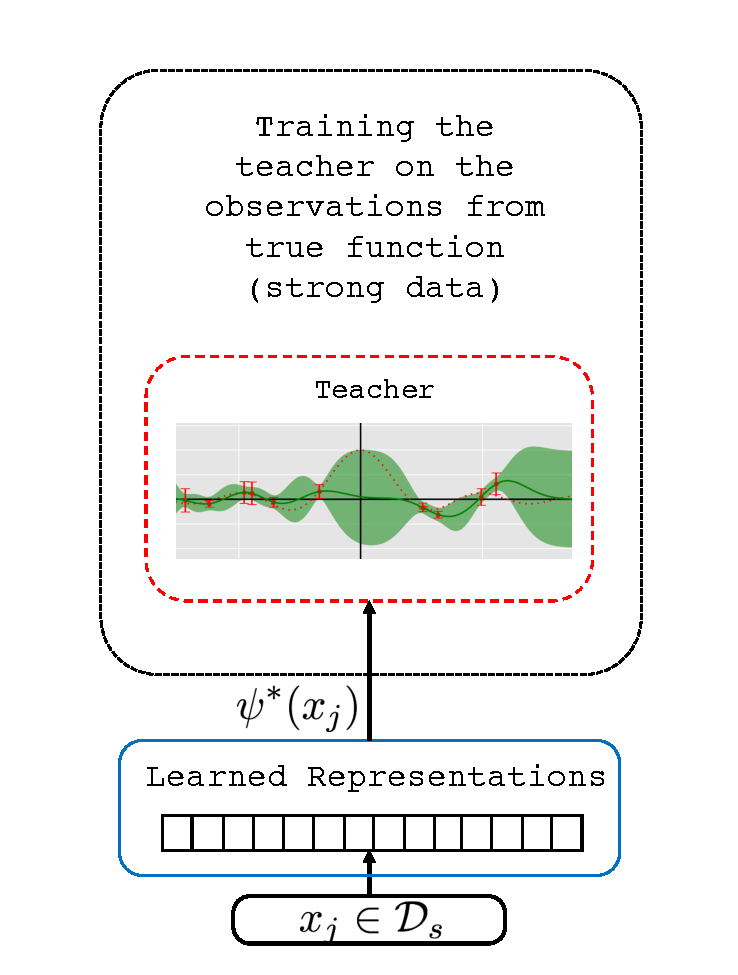
\includegraphics[width=\textwidth]{03-part-02/chapter-05/figs_and_tables/fig_fwl_step_2.pdf}
        \caption{\label{fig:step2}Step 2}
    \end{subfigure}%
     ~
    \begin{subfigure}[t]{0.425\textwidth}
        \centering
        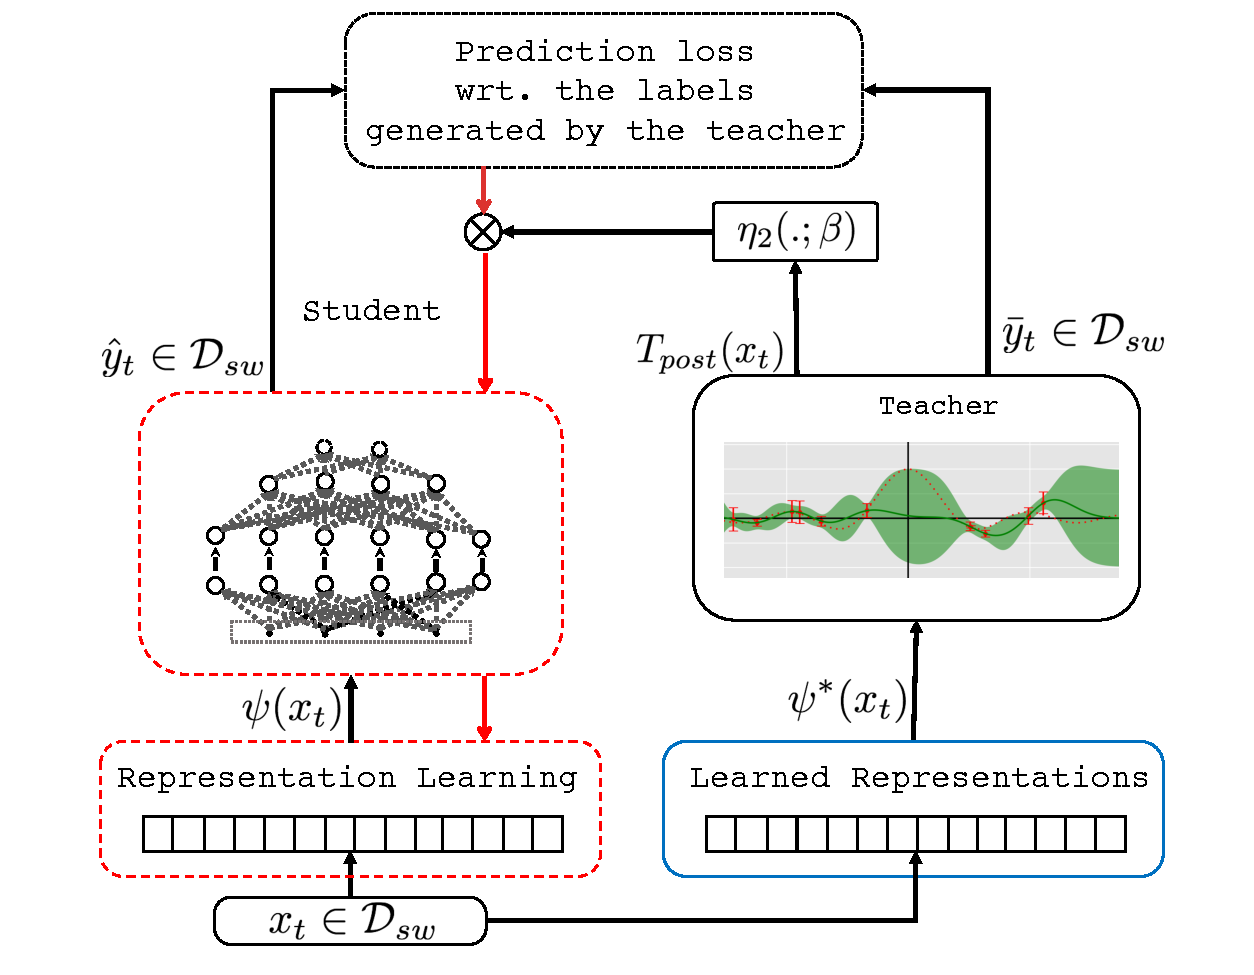
\includegraphics[width=\textwidth]{03-part-02/chapter-05/figs_and_tables/fig_fwl_step_3.pdf}
        \caption{\label{fig:step3}Step 3}
    \end{subfigure}%
    }
    \caption{Illustration of \fwlfull: Step 1: Pre-train \std on weak data,  Step 2: Fit \tch to observations from the true function, and Step 3: Fine-tune \std on labels generated by \tch, taking the confidence into account. Red dotted borders and blue solid borders depict components with trainable and non-trainable parameters, respectively.}
    \label{fig:model_fwl}
\end{figure}
\subsection{Recipe of the \fwlfull}
\label{sec:proposed-method}
In this section, we describe the \fwl approach for semi-supervised learning when we have access to weak supervision (e.g., heuristics or weak annotators). 

Our proposed setup comprises a neural network called the \textbf{\std} and a Bayesian function approximator called the \textbf{\tch}. The training process consists of three phases which we summarize in Algorithm~\ref{alg:fwl:main} and Figure~\ref{fig:model_fwl}.

\textbf{Step 1} \emph{Pre-train the \std on $\mathcal{D}_w$ using weak labels generated by the \wa}. 

The main goal of this step is to learn a \emph{task dependent} representation of the data as well as pretraining the \std. The \std function is a neural network consisting of two parts. The first part $\psi(.)$ learns the data representation and the second part $\phi(.)$ performs the prediction task (e.g., classification). Therefore the overall function is $\hat{y}=\phi(\psi(x_i))$. The \std is trained on all samples of the weak dataset $\mathcal{D}_w=\{(x_i, \tilde{y}_i)\}$. For brevity, in the following, we will refer to both data sample $x_i$ and its representation $\psi(x_i)$ by $x_i$ when it is obvious from the context. 
From the self-supervised feature learning point of view, we can say that representation learning in this step is solving a surrogate task of approximating the expert knowledge, for which a noisy supervision signal is provided by the \wa.  


\textbf{Step 2} \emph{Train the \tch on the strong data $(\psi(x_j),y_j) \in \mathcal{D}_s$ represented in terms of the student representation $\psi(.)$ and then use the \tch to generate a soft dataset $\mathcal{D}_{sw}$ consisting of $\langle \textrm{sample}, \textrm{predicted label}, \textrm{ confidence} \rangle$ for \textbf{all} data samples.} 

We use a Gaussian process as the \tch to capture the label uncertainty in terms of the \std representation, estimated w.r.t\ the strong data. A prior mean and co-variance function is chosen for $\mathcal{GP}$. The learned embedding function $\psi(\cdot)$ in Step 1 is then used to map the data samples to dense vectors as input to the $\mathcal{GP}$. 
We use the learned representation by the \std in the previous step to compensate lack of data in $\mathcal{D}_s$ and the \tch can enjoy the learned knowledge from the large quantity of the weakly annotated data. This way, we also let the \tch  see the data through the lens of the \std.

The $\mathcal{GP}$ is trained on the samples from $\mathcal{D}_s$ to learn the posterior mean $\bm{m}_{\rm post}$ (used to generate soft labels) and posterior co-variance $K_{\rm post}(.,.)$ (which represents label uncertainty).
%\begin{eqnarray*}
%\mathcal{GP}(\bm{m}_{\rm post}, K_{\rm post})&=&\mathcal{GP}(\bm{m}_{\rm %prior}, K_{\rm prior}) | \mathcal{D}_s=\{(\psi(x_j),y_j)\}\\
%\sshrink
%\end{eqnarray*}
We then create the \emph{soft dataset} $\mathcal{D}_{sw}=\{(x_t,\bar{y}_t)\}$ using the posterior $\mathcal{GP}$, input samples $x_t$ from $\mathcal{D}_w \cup \mathcal{D}_s$, and predicted labels $\bar{y}_t$ with their associated uncertainties as computed by $T(x_t)$ and $\Sigma(x_t)$:
\begin{eqnarray*}
\tfunc(x_t) &=& g(\bm{m}_{\rm post}(x_t))\\
\Sigma(x_t) &=& h(K_{\rm post}(x_t,x_t))
\sshrink
\end{eqnarray*}
The generated labels are called \emph{soft labels}. Therefore, we refer to $\mathcal{D}_{sw}$ as a soft dataset. $g(.)$ transforms the output of $\mathcal{GP}$ to the suitable output space. For example, in classification tasks, $g(.)$ would be the softmax function to produce probabilities that sum up to one. 
For multidimensional-output tasks where a vector of variances is provided by the $\mathcal{GP}$, the vector $K_{\rm post}(x_t,x_t)$ is passed through an aggregating function $h(.)$ to generate a scalar value for the uncertainty of each sample. 
Note that we train $\mathcal{GP}$ only on the strong dataset $\mathcal{D}_s$ but then use it to generate soft labels $\bar{y}_t = \tfunc(x_t)$ and uncertainty $\Sigma(x_t)$ for samples belonging to $\mathcal{D}_{sw}=\mathcal{D}_w\cup \mathcal{D}_s$.

In practice, we furthermore divide the space of data into several regions and assign each region a separate $\mathcal{GP}$ trained on samples from that region. This leads to a better exploration of the data space and makes use of the inherent structure of data. The algorithm called clustered $\mathcal{GP}$ gave better results compared to a single GP. 

By this division of space, we take advantage of the knowledge learned by several teachers, each an expert on its specific region of data space, which helps in particular when the dimensionality of the input is rather high. As a nice side-effect, this also solves the scalability issues of $\mathcal{GP}$s in that we can increase the number of regions until the number of points in each region is tractable with a single $\mathcal{GP}$, and train these models in parallel. See Section~\ref{sec:CGP} for the detailed description of clustered $\mathcal{GP}$.

\setlength{\textfloatsep}{10pt}
\begin{algorithm}[t!]
\small
% \fontsize{9}{11}\selectfont
\caption{\fwlfull.}%, 
\begin{algorithmic}[1]
\label{alg:main}

\State Train the \std on samples from the weakly-annotated data $D_w$.
\medskip
\State Freeze the representation-learning component $\psi(.)$ of the \std and train \tch on the strong data $D_s={(\psi(x_j),y_j)}$. Apply \tch to unlabeled samples $x_t$ to obtain soft dataset $D_{sw}=\{(x_t, \bar{y}_t)\}$ where $\bar{y}_t=T(x_t)$ is the soft label and for each instance $x_t$, the uncertainty of its label, $\Sigma(x_t)$, is provided by the \tch.
\medskip
\State Train the \std on samples from $D_{sw}$ with SGD and modulate the step-size $\eta_t$ according to the per-sample quality estimated using the \tch (Equation~\ref{eqn:eta2}).
\end{algorithmic}
\end{algorithm}

%
\textbf{Step 3} \emph{Fine-tune the weights of the \std network on the soft dataset, while modulating the magnitude of each parameter update by the corresponding \tch-confidence in its label.}

The \std network of Step 1 is fine-tuned using samples from the soft dataset $\mathcal{D}_{sw}=\{(x_t, \bar{y}_t)\}$ where $\bar{y}_t=\tfunc(x_t)$.
The corresponding uncertainty $\Sigma(x_t)$ of each sample is mapped to a confidence value according to Equation~\ref{eqn:eta2} below, and this is then used to determine the step size for each iteration of the stochastic gradient descent (SGD). So, intuitively, for data points where we have true labels, the uncertainty of the \tch is almost zero, which means we have high confidence and a large step-size for updating the parameters. However, for data points where the \tch is not confident, we down-weight the training steps of the \std. This means that at these points, we keep the \std function as it was trained on the weak data in Step 1.

More specifically, we update the parameters of the \std by training on $\mathcal{D}_{sw}$ using SGD:
\begin{eqnarray*}
%  \pmb{w}^* &=& \argmin_{\pmb{w} \in \mathcal{W}} \>   \mathcal{L}(\pmb{w}) \\
%  &:=& \frac{1}{T}\sum_{(x_t,\bar{y}_t) \in \mathcal{D}_{sw}}l(\pmb{w}, x_i, \bar{y}_i) + \mathcal{R}(\pmb{w}), \\
  \pmb{w}^* &=& \argmin_{\pmb{w} \in \mathcal{W}} \> \frac{1}{N}\sum_{(x_t,\bar{y}_t) \in \mathcal{D}_{sw}}l(\pmb{w}, x_t, \bar{y}_t) + \mathcal{R}(\pmb{w}), \\
  \pmb{w}_{t+1} &=& \pmb{w}_t - \eta_t(\nabla l(\pmb{w},x_t,\bar{y}_t) + \nabla \mathcal{R}(\pmb{w}))
\end{eqnarray*}
where $l(\cdot)$ is the per-sample loss, $\eta_t$ is the total learning rate, $N$ is the size of the soft dataset $\mathcal{D}_{sw}$, $\pmb{w}$ is the parameters of the \std network, and $\mathcal{R(.)}$ is the regularization term. %Regularization term is the usual regularization used by optimization packages (e.g., weight decay). Therefore, we do not go into its details here.

We define the total learning rate as $\eta_t = \eta_1(t)\eta_2(x_t)$, where $\eta_1(t)$ is the usual learning rate of our chosen optimization algorithm that anneals over training iterations, and $\eta_2(x_t)$ is a function of the label uncertainty $\Sigma(x_t)$ that is computed by the \tch for each data point. Multiplying these two terms gives us the total learning rate. In other words, $\eta_2$ represents the \emph{fidelity} (quality) of the current sample, and is used to multiplicatively modulate $\eta_1$. Note that the first term does not necessarily depend on each data point, whereas the second term does. We propose
\begin{equation}
 \label{eqn:eta2}
 \eta_2(x_t) = \exp[-\beta \Sigma(x_t)],    
\end{equation}
to exponentially decrease the learning rate for data point $x_t$ if its corresponding soft label $\bar{y}_t$ is unreliable (far from a true sample).
In practice, when using mini-batches, we implement this by multiplying the loss of each sample in the batch by its fidelity score and average over these fidelity-weighted losses in the batch when calculating the batch gradient based on that loss. In Equation~\ref{eqn:eta2}, $\beta$ is a positive scalar hyper-parameter. Intuitively, small $\beta$ results in a \std which listens more carefully to the \tch and copies its knowledge, while a large $\beta$ makes the \std pay less attention to the \tch, staying with its initial weak knowledge. 
More concretely speaking, as $\beta \to 0$ \std places more trust in the labels $\bar{y}_t$ estimated by the \tch and the \std copies the knowledge of the \tch. On the other hand, as $\beta \to \infty$, \std puts less weight on the extrapolation ability of $\mathcal{GP}$ and the parameters of the \std are not affected by the correcting information from the \tch. 


\subsection{Multi-Teacher \fwl using Clustered GP}
\label{sec:CGP}
In this section, we explain the clustered GP which is an effective way of applying GP where the scale of the data increases.  Clustered GP suggests using several $\mathcal{GP}=\{GP_{c_i}\}$ to explore the entire data space more effectively. Even though inducing points and stochastic methods make $\mathcal{GP}$s more scalable we still observed poor performance when the entire dataset was modeled by a single $\mathcal{GP}$. Therefore, the reason for using multiple $\mathcal{GP}$s is mainly empirical inspired by ~\citep{shen2006fast} which is explained in the following:

We used Sparse Gaussian Process implemented in GPflow. The algorithm is scalable in the sense that it is not $O(N^3)$ as original $\mathcal{GP}$ is. It introduces inducing points in the data space and defines a variational lower bound for the marginal likelihood. The variational bound can now be optimized by stochastic methods which make the algorithm applicable in large datasets. However, the tightness of the bound depends on the location of inducing points which are found through the optimization process. 

We empirically observed that a single $\mathcal{GP}$ does not give a satisfactory accuracy on left-out test dataset. We hypothesized that this can be due to the inability of the algorithm to find good inducing points when the number of inducing points is restricted to just a few.
Then we increased the number of inducing points $M$ which trades off the scalability of the algorithm because it scales with $O(NM^2)$. Moreover, apart from scalability which is partly solved by stochastic methods, we argue that the structure of the entire space may not be explored well by a single $\mathcal{GP}$ and its inducing points.
We guess this can be due to the observation that our datasets are distributed in a highly sparse way within the high dimensional embedding space. 
We also tried to cure the problem by means of PCA to reduce input dimensions and give a denser representation, but it did not result in a considerable improvement\citep{dehghani:2018:ICLR}. 
%The results are presented in Tabel~\ref{tbl_cgp}. 
%\input{cgp_res.tex}

We may be able to argue that clustered $\mathcal{GP}$ makes better use of the data structure roughly close to the idea of KISS-GP~\citep{Wilson:2015:KIS:3045118.3045307}.
In inducing point methods, it is normally assumed that $M\ll N$ ($M$ is the number of inducing points and $N$ is the number of training samples) for computational and storage saving. However, we have this intuition that few number of inducing points make the model unable to explore the inherent structure of data. By employing several GPs, we were able to use a large number of inducing points even when $M>N$ ($M$ is the total number of inducing points) which seemingly better exploits the structure of datasets. Because our work was not aimed to be a close investigation of GP, we considered clustered $\mathcal{GP}$ as the engineering side of the work which is a tool to give us a measure of confidence. Other tools such as a single $\mathcal{GP}$ with inducing points that form a Kronecker or Toeplitz covariance matrix are also conceivable. Therefore, we do not of course claim that we have proposed a new method of inference for GPs. 

Here is practical description of clustered $\mathcal{GP}$ algorithm:\\
{\it Clustered $\mathcal{GP}$}: Let $N$ be the size of the dataset on which we train the \tch. Assume we allocate $K$ teachers to the entire data space. Therefore, each $\mathcal{GP}$ sees a dataset of size $n=N/K$.
Then we use a simple clustering method (e.g., k-means) to find centroids of $K$ clusters $C_1, C_2, \ldots, C_K$ where $C_i$ consists of samples $\{x_{i,1}, x_{i,2},\ldots,x_{i,n}\}$. We take the centroid $c_i$ of cluster $C_i$ as the representative sample for all its content. Note that $c_i$ does not necessarily belong to $\{x_{i,1}, x_{i,2},...,x_{i,n}\}$. We assign each cluster a $\mathcal{GP}$ trained by samples belonging to that cluster. More precisely, cluster $C_i$ is assigned a $\mathcal{GP}$ whose data points are $\{x_{i,1}, x_{i,2},...,x_{i,n}\}$.
Because there is no dependency among different clusters, we train them in parallel to speed-up the procedure more. 

The pseudo-code of the clustered $\mathcal{GP}$ is presented in Algorithm~\ref{alg:CGP}. When the main issue is computational resources (when the number of inducing points for each $\mathcal{GP}$ is large), we can first choose the number $n$ which is the maximum size of the dataset on which our resources allow to train a $\mathcal{GP}$, then find the number of clusters $K=N/n$ accordingly. The rest of the algorithm remains unchanged. 
\begin{algorithm}[t!]
% \small
\caption{Clustered Gaussian processes.}%, 
\begin{algorithmic}[1]
\label{alg:CGP}
\State Let $N$ be the sample size, $n$ the sample size of each cluster, $K$ the number of clusters, and $c_i$ the center of cluster $i$.
\medskip
\State Run K-means with $K$ clusters over all samples with true labels $\mathcal{D}_s=\{x_i,y_i\}$.
\begin{equation*}
    {\rm K\mbox{-}means}({x_i}) \rightarrow {c_1, c_2, \ldots, c_K}
\end{equation*}
where $c_i$ represents the center of cluster $C_i$ containing samples $D_s^{c_i}=\{x_{i,1}, x_{i,2}, ... x_{i,n}\}$.
\medskip
\State Assign each of $K$ clusters a Gaussian process and train them in parallel to approximate the label of each sample.
\begin{eqnarray*}
\mathcal{GP}_{c_i}(\bm{m}_{\rm post}^{c_i}, K_{\rm post}^{c_i})&=&\mathcal{GP}(\bm{m}_{\rm prior}, K_{\rm prior}) | D_s^{c_i}=\{(\psi(x_{s,c_i}),y_{s,c_i})\}\\
\tfunc_{c_i}(x_t) &=& g(\bm{m}_{\rm post}^{c_i}(x_t))\\
\Sigma_{c_i}(x_t) &=& h(K_{\rm post}^{c_i}(x_t,x_t))
\end{eqnarray*}



% \tfunc_{{\rm prior},{c_i}}&=&\mathcal{GP}_{c_i}(\bm{0}, K_{\rm prior})\\
% T_{c_i}|\mathcal{D}_s^{c_i}, \tfunc{\rm prior }&=&\mathcal{GP}_{c_i}(\bm{m}_{{\rm prior}, {c_i}}, K_{\rm prior})

where $\mathcal{GP}_{c_i}$ is trained on $\mathcal{D}_s^{c_i}$ containing samples belonging to the cluster $c_i$. Other elements are defined in Section~\ref{sec:proposed-method}
\medskip
\State Use trained teacher $\tfunc_{c_i}(.)$ to evaluate the soft label and uncertainty for samples from $\mathcal{D}_{sw}$ to compute $\eta_2(x_t)$ required for step 3 of Algorithm~\ref{alg:main}. We use $\tfunc(.)$ as a wrapper for all teachers $\{T_{c_i}\}$.
\end{algorithmic}
\end{algorithm}
\shrink



\subsection{FWL on a Toy Example}
\label{sec:toy_exmpale}
\begin{figure}[!t]%
   \makebox[\linewidth][c]{%
    \centering
    \begin{subfigure}[t]{0.5\textwidth}
        \centering
        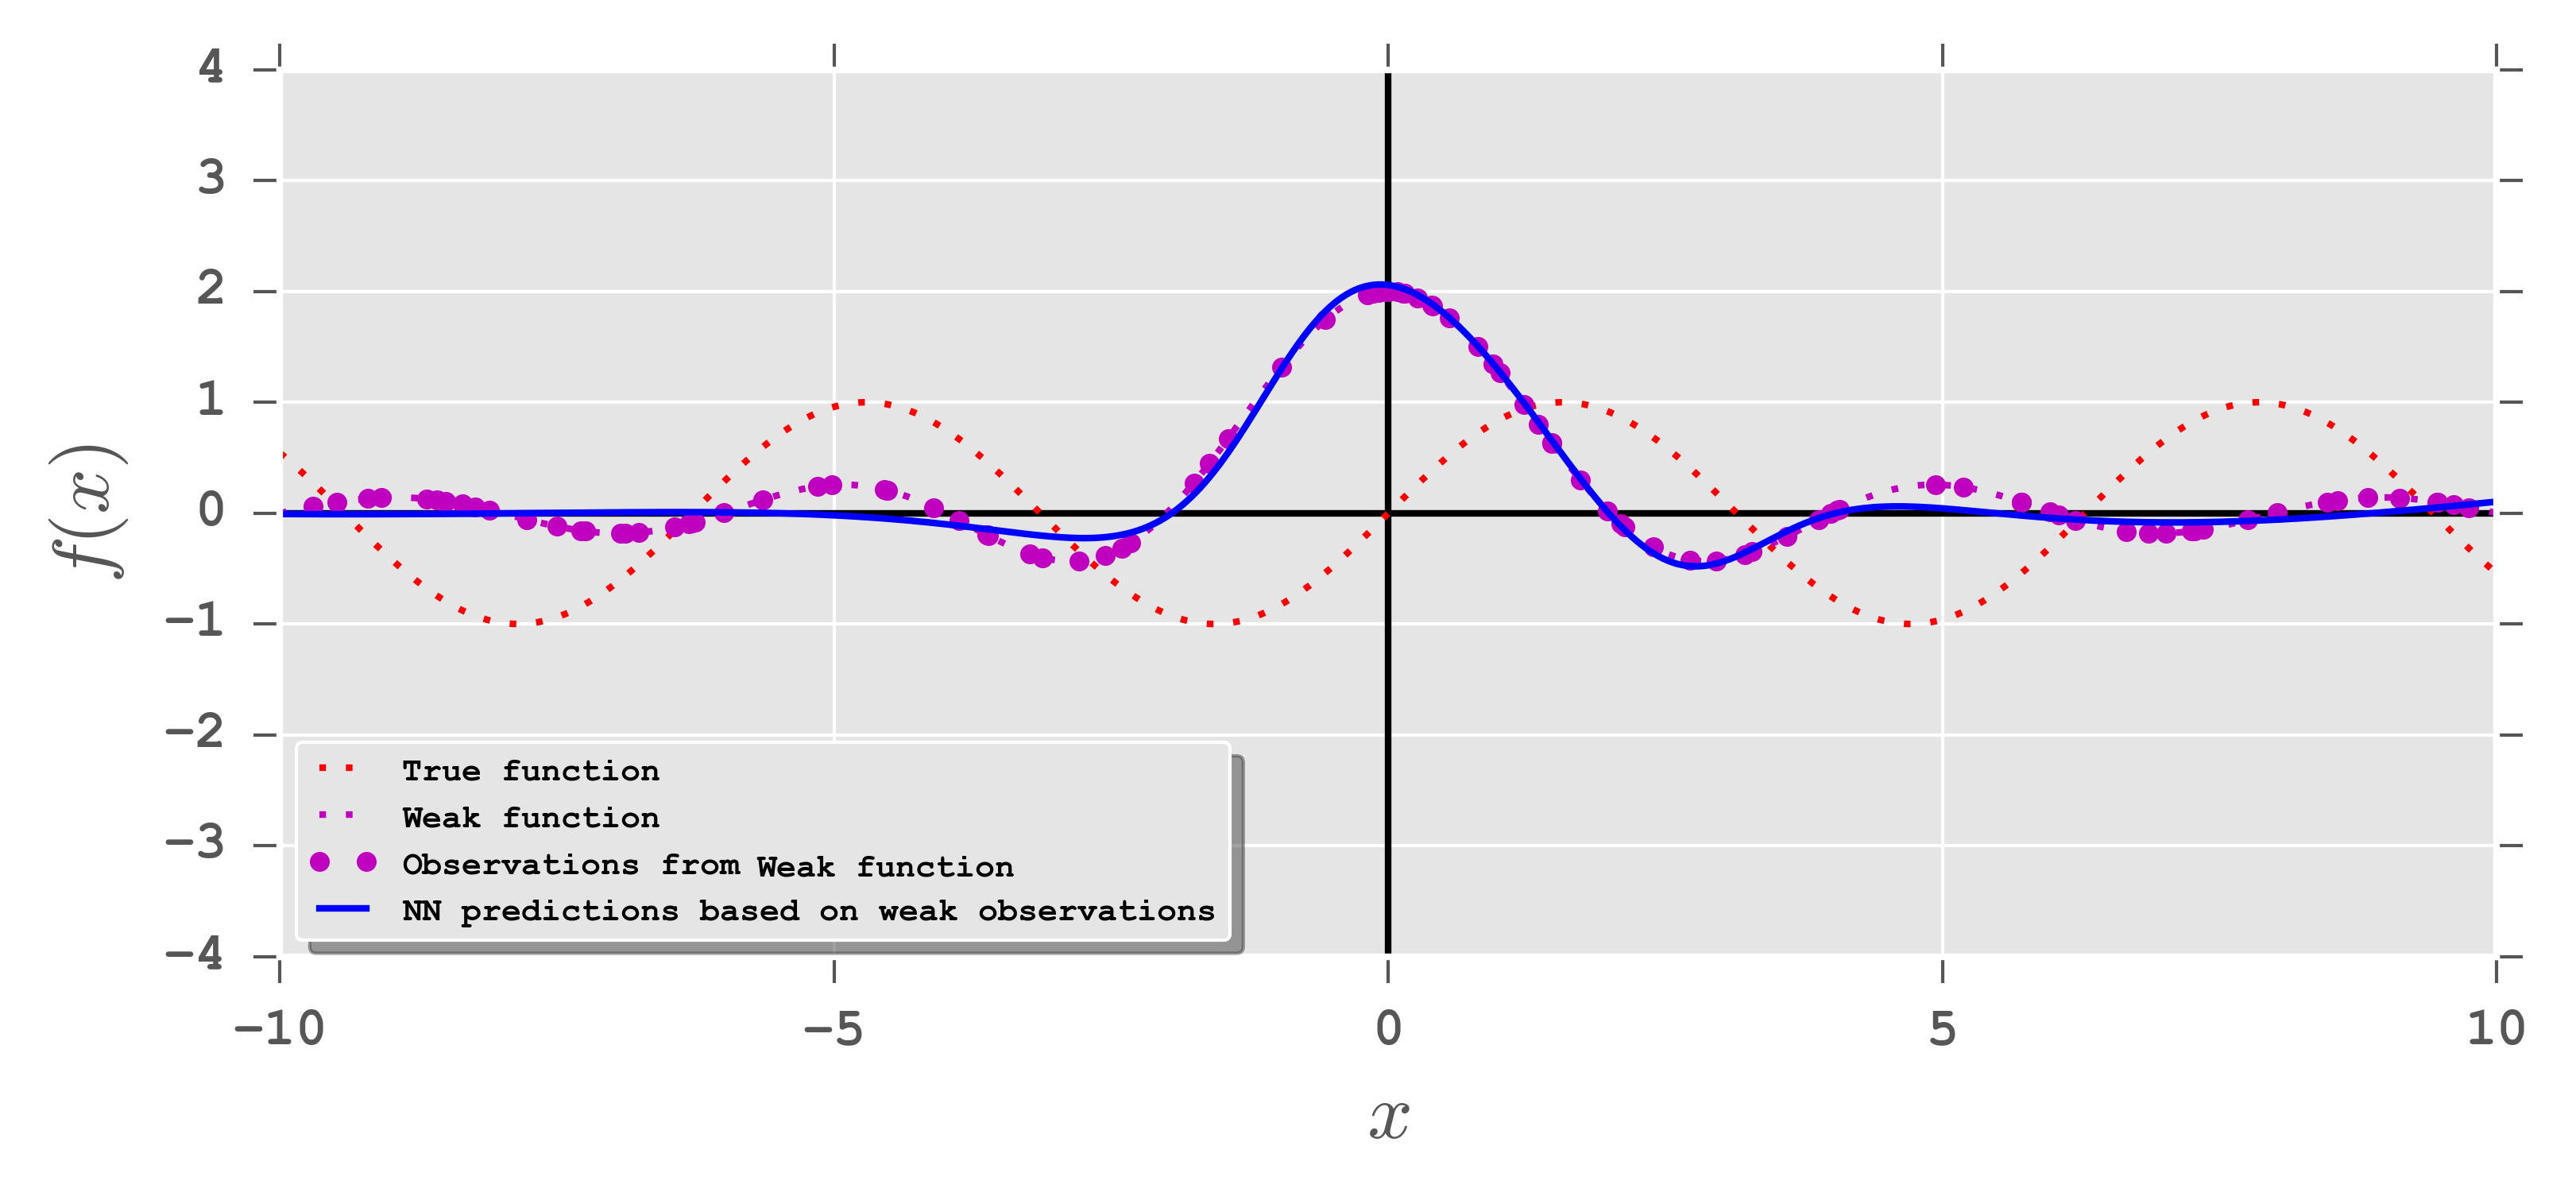
\includegraphics[width=1\textwidth]{03-part-02/chapter-05/figs_and_tables/fig_toy_ex_plot1.png}
        \caption{\label{fig:toy_plot1}Training \std on 100 samples from the weak function.}
    \end{subfigure}%
    ~
    \begin{subfigure}[t]{0.5\textwidth}
        \centering
        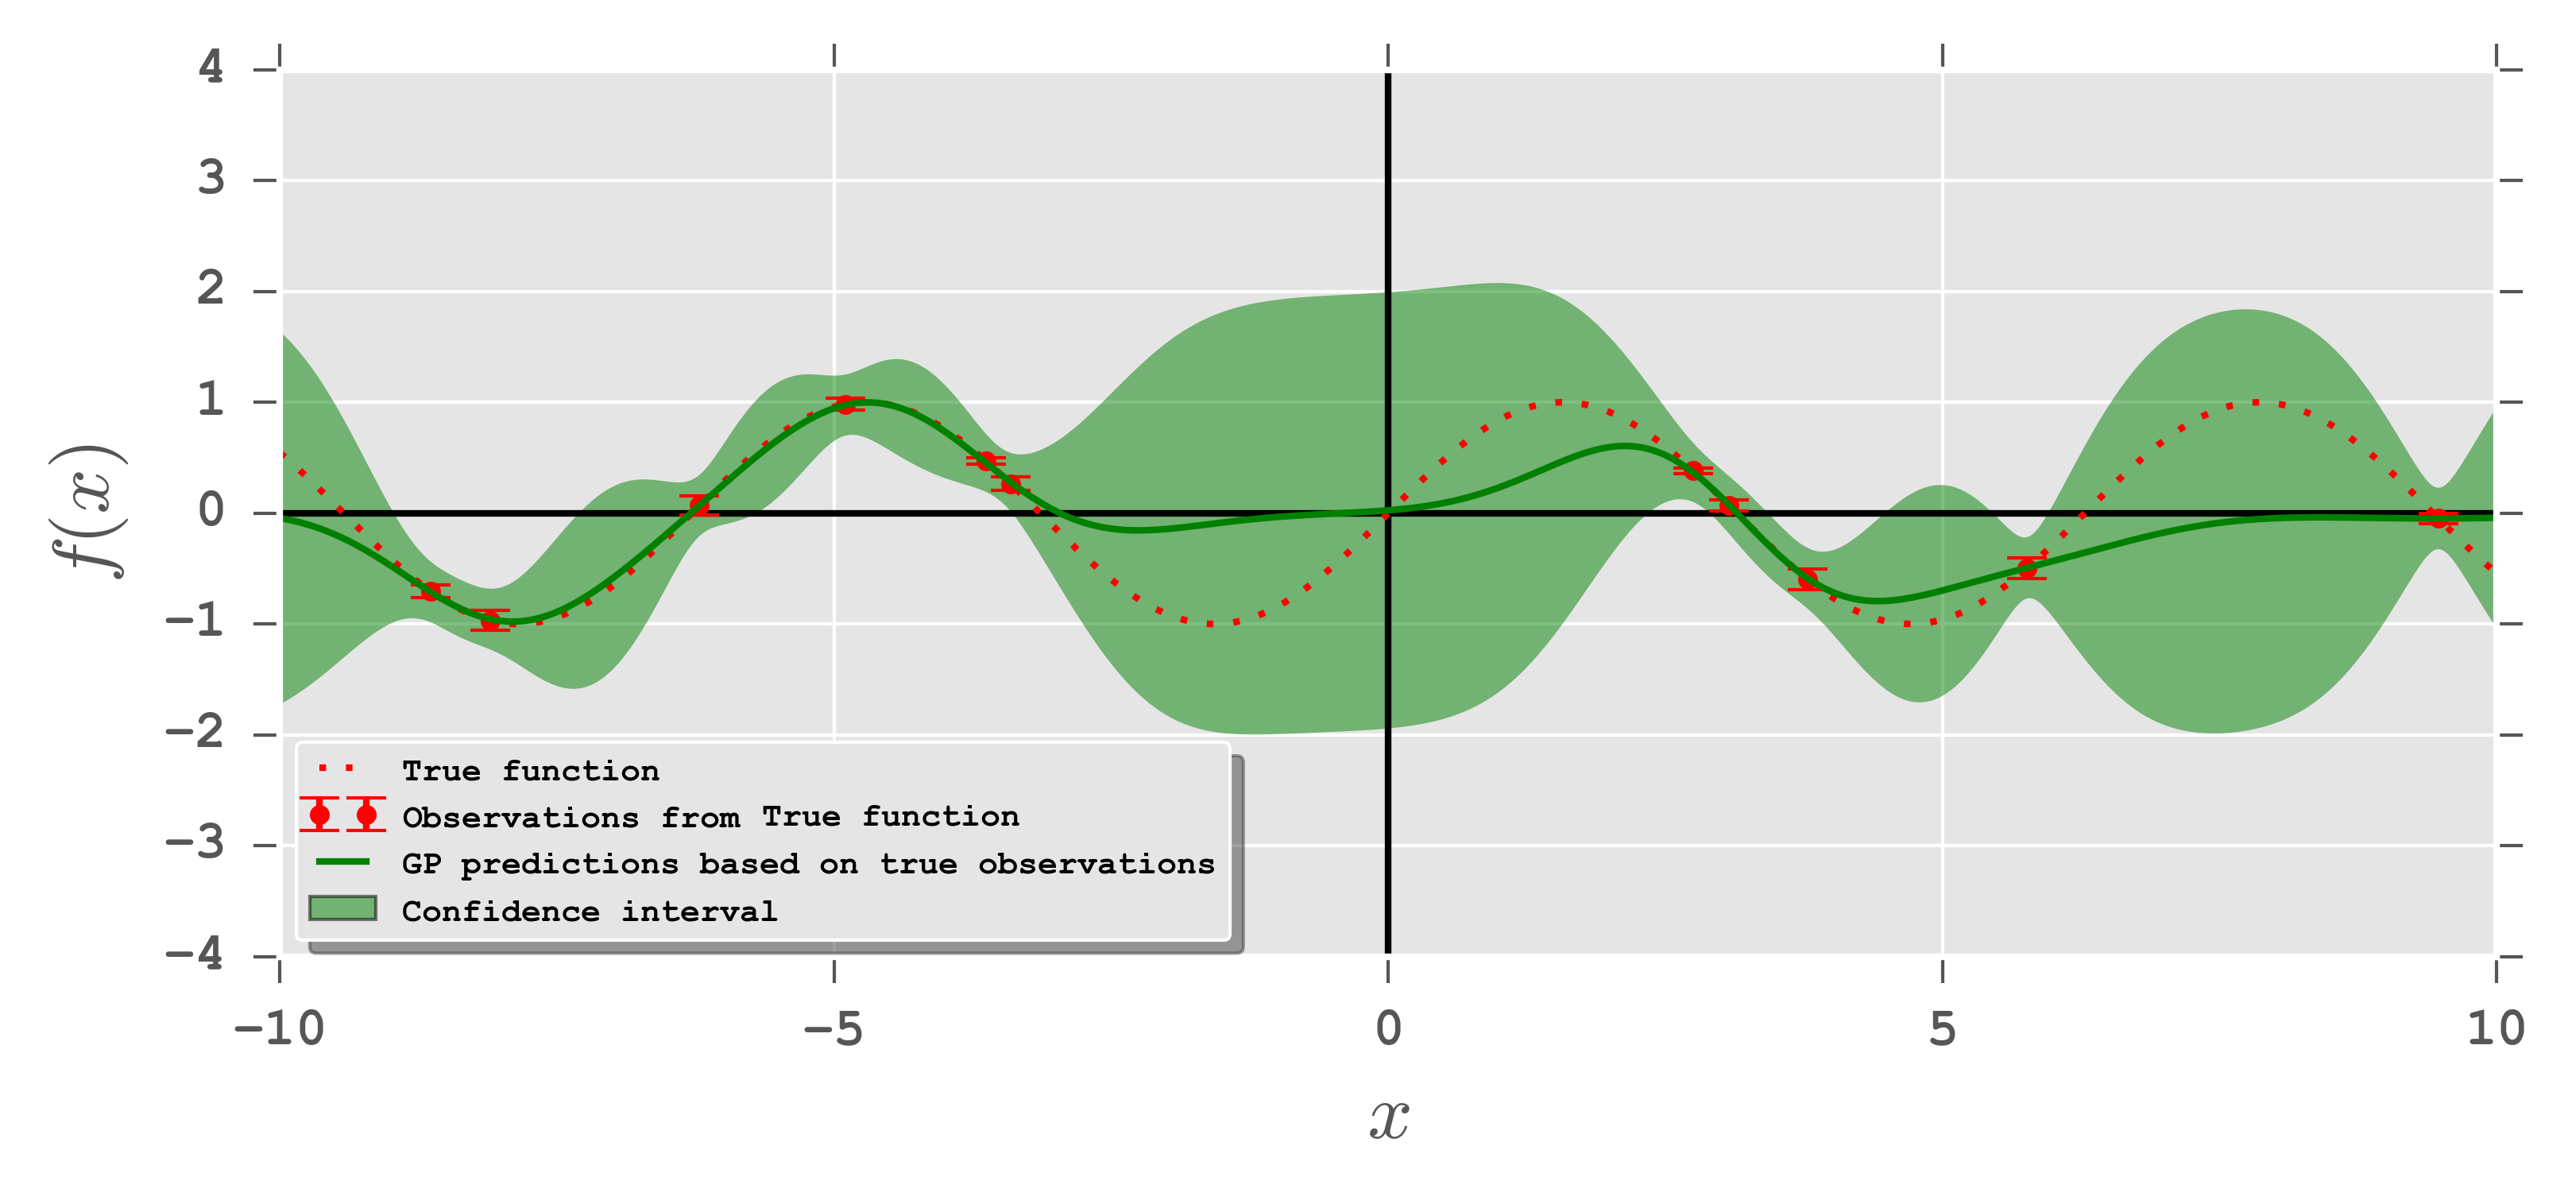
\includegraphics[width=1\textwidth]{03-part-02/chapter-05/figs_and_tables/fig_toy_ex_plot2.png}
        \caption{\label{fig:toy_plot2}Fitting \tch based on 10 observations from the true function.}
    \end{subfigure}%
    }
    \\
    \makebox[\linewidth][c]{%
    \begin{subfigure}[t]{0.5\textwidth}
        \centering
        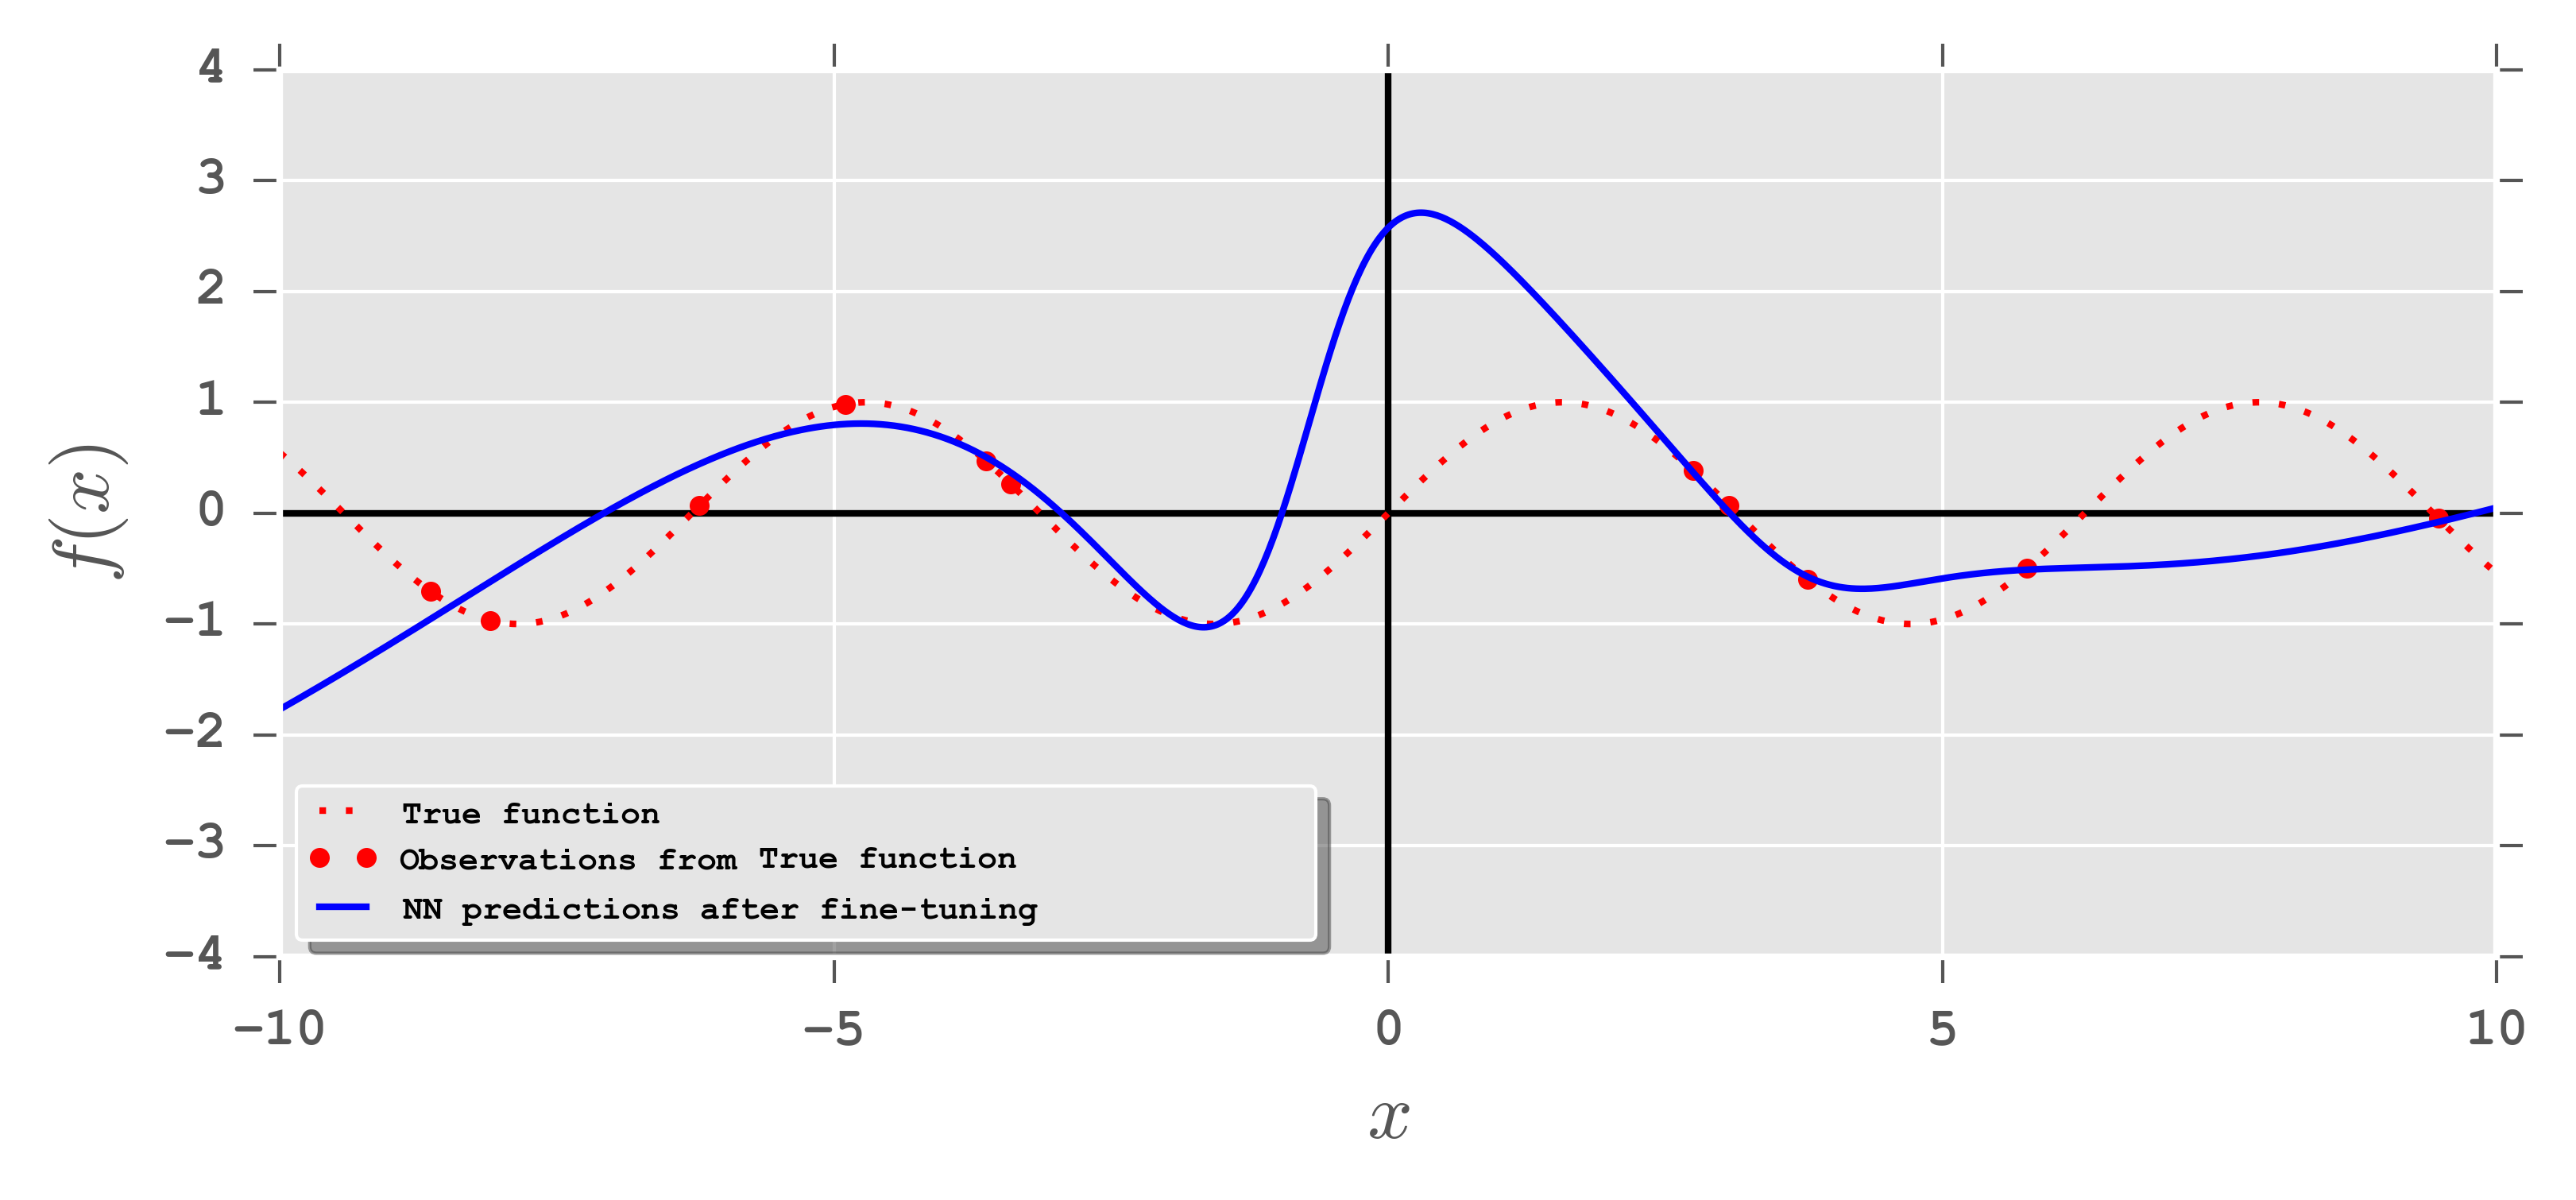
\includegraphics[width=1\textwidth]{03-part-02/chapter-05/figs_and_tables/fig_toy_ex_plot3.png}
        \caption{\label{fig:toy_plot3}Fine-tuning the \std based on observations from the true function.}
    \end{subfigure}%
    ~
    \begin{subfigure}[t]{0.5\textwidth}
        \centering
        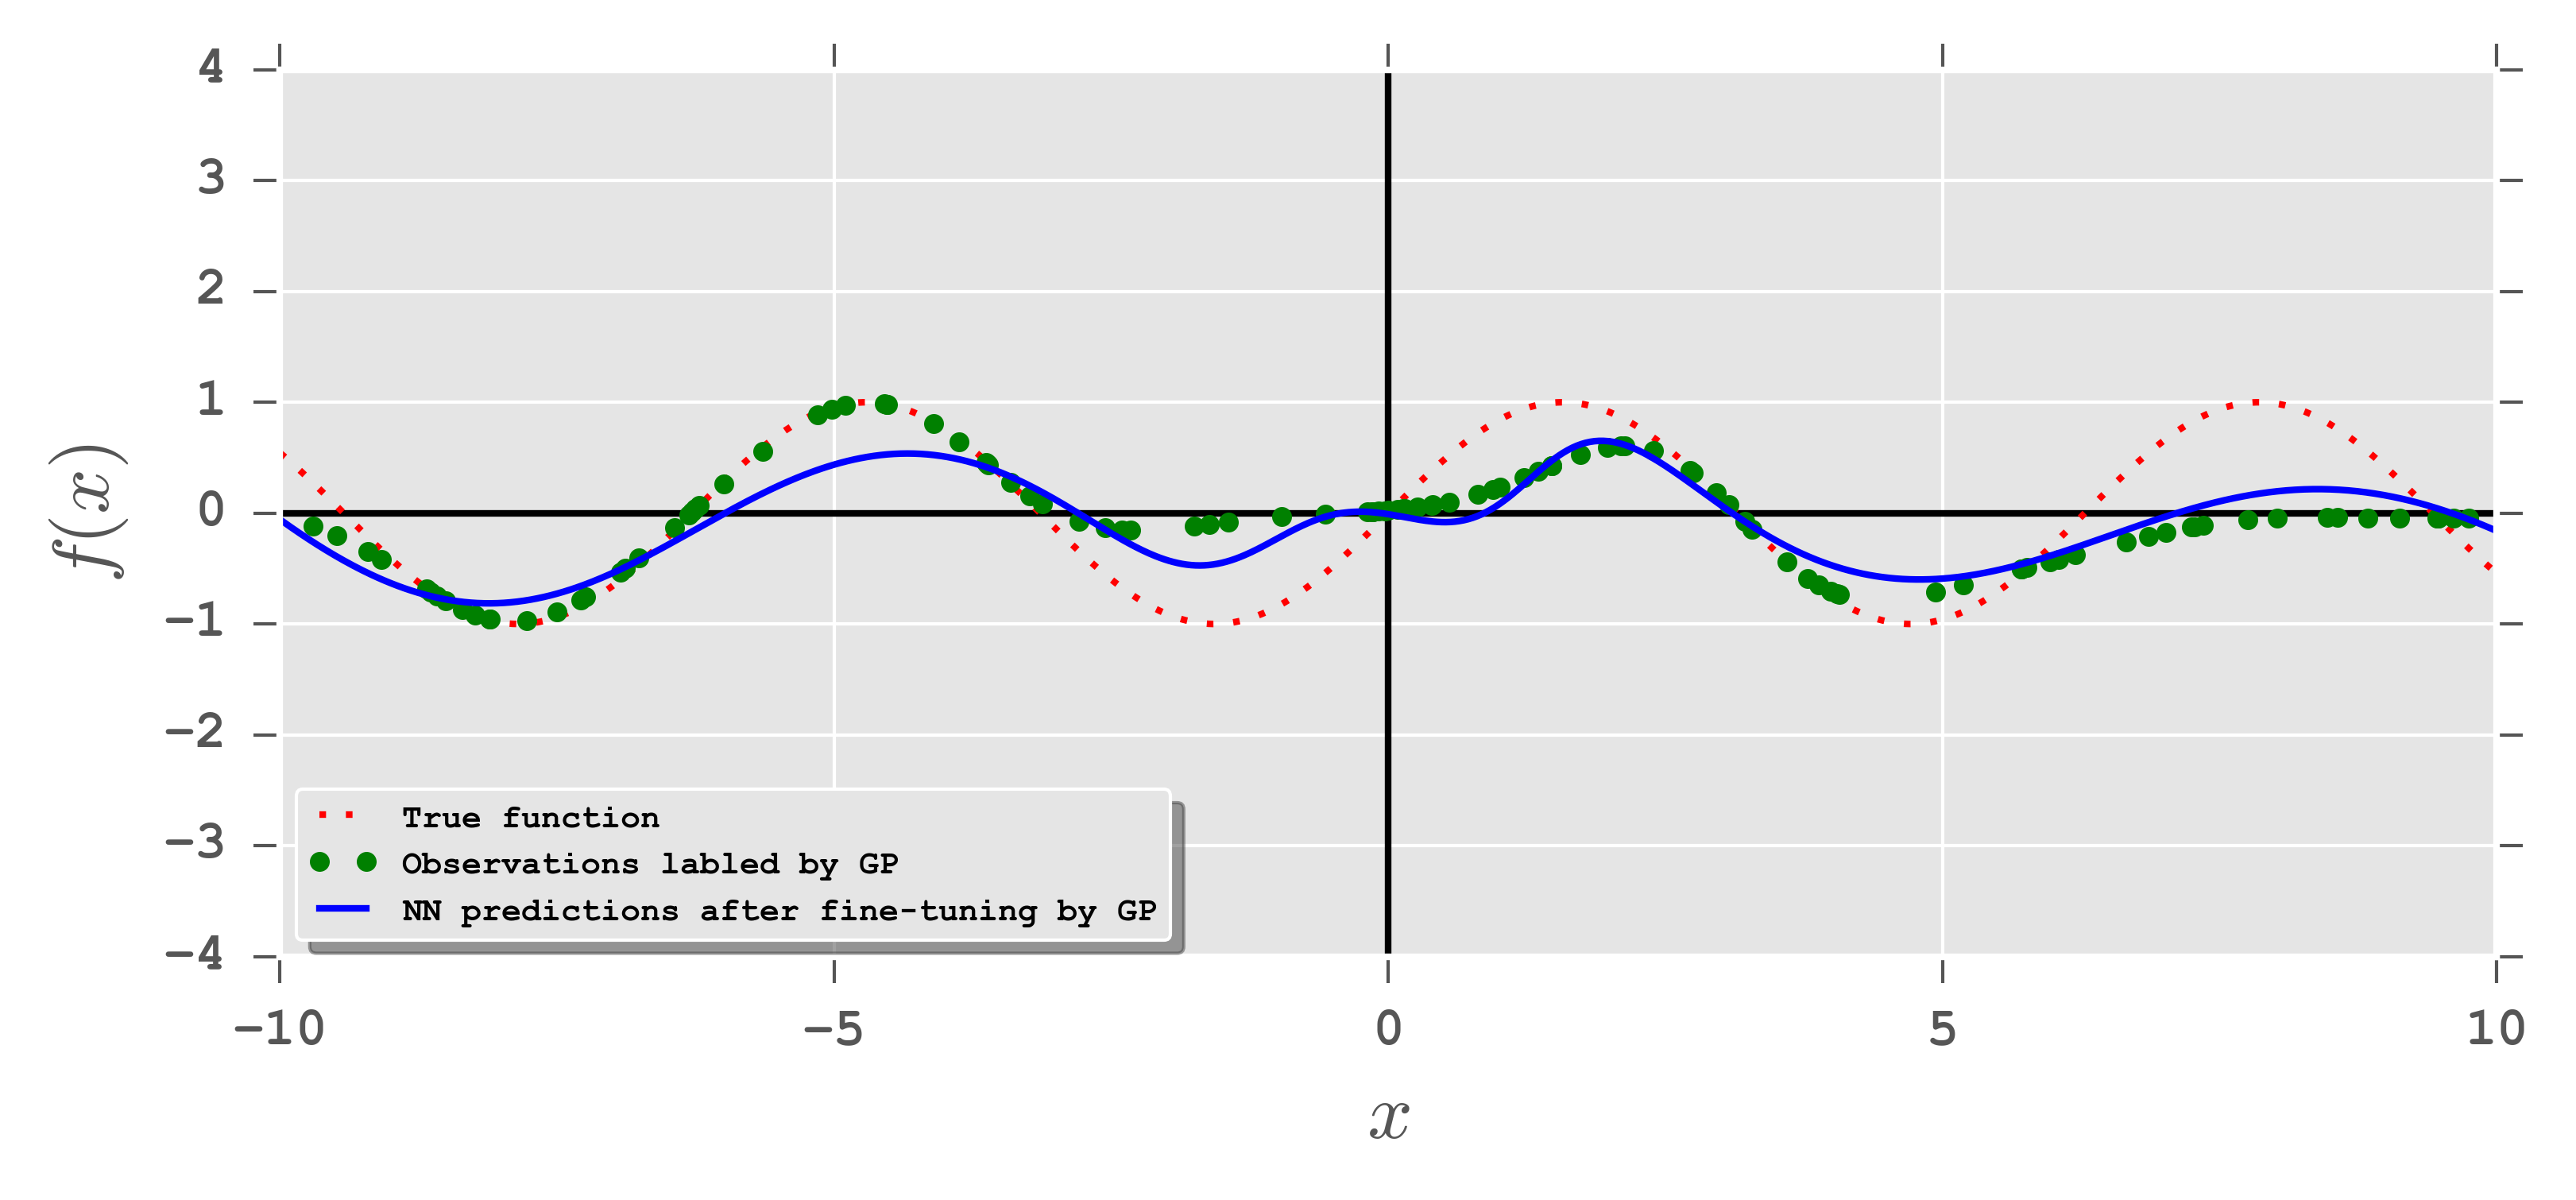
\includegraphics[width=1\textwidth]{03-part-02/chapter-05/figs_and_tables/fig_toy_ex_plot4.png}
        \caption{\label{fig:toy_plot4}Fine-tuning the \std based on label/confidence from \tch.}
    \end{subfigure}%
    }
    \vspace{-5pt}
    \caption{Toy example: The true function we want to learn is $y = \sin(x)$ and the weak function is $y = 2 sinc(x)$.}
    \label{fig:toy}
    \vspace{-5pt}
\end{figure}
To better understand \fwl, we apply \fwl to a one-dimensional toy problem to illustrate the various steps.
%
Let $f_t(x)=\sin(x)$ be the true function (red dotted line in Figure~\ref{fig:toy_plot1}) from which a small set of observations $\mathcal{D}_s=\{x_j,y_j\}$ is provided (red points in Figure~\ref{fig:toy_plot2}). These observation might be noisy, in the same way that labels obtained from a human labeler could be noisy.
%
A \wa function $f_{w}(x)=2sinc(x)$ (magenta line in Figure~\ref{fig:toy_plot1}) is provided, as an approximation to $f_t(.)$.

%
The task is to obtain a good estimate of $f_t(.)$ given the set $\mathcal{D}_s$ of strong observations and the \wa function $f_{w}(.)$.
%
We can easily obtain a large set of observations $\mathcal{D}_w=\{x_i,\tilde{y}_i\}$ from $f_{w}(.)$ with almost no cost (magenta points in Figure~\ref{fig:toy_plot1}). 

As the \tch, we use standard Gaussian process regression\footnote{\url{http://gpflow.readthedocs.io/en/latest/notebooks/regression.html}} with this kernel:
\begin{equation}
k(x_i,x_j)=k_{\rm RBF}(x_i,x_j)+k_{\rm White}(x_i,x_j)
\end{equation}
where,
\begin{flalign*}
    \hspace{6em}
    &&k_{\rm RBF}(x_i,x_j) &= \exp{\left(\frac{\Vert x_i-x_j\Vert^2}{2^2}\right)} & 
    \\
    &&k_{\rm White}(x_i,x_j) &= constant\_value, \quad \forall x_1=x_2 \text{ and } 0 \text{ otherwise} & 
\end{flalign*}

We fit only one $\mathcal{GP}$ on all the data points (i.e., no clustering). Also during fine-tuning, we set $\beta = 1$.
The \std is a simple feed-forward network with the depth of 3 layers and width of 128 neurons per layer.  We have used $tanh$ as the nonlinearity for the intermediate layers and a linear output layer. As the optimizer, we used Adam~\citep{Kingma:2014} and the initial learning rate has been set to $0.001$.
We randomly sample 100 data points from the \wa and 10 data points from the true function. We introduce a small amount of noise to the observation of the true function to model the noise in the human labeled data. 


We consider two experiments: 
\begin{enumerate}[leftmargin=*]
%save some space
\setlength{\topsep}{0.3pt}
\setlength{\partopsep}{0.3pt}
\setlength{\itemsep}{0.3pt}
\setlength{\parskip}{0.3pt}
\setlength{\parsep}{0.3pt}
    \item A neural network trained on weak data and then fine-tuned on strong data from the true function, which is the most common semi-supervised approach (Figure~\ref{fig:toy_plot3}).
    \item A teacher-student framework working by the proposed \fwl approach.
\end{enumerate} 

As can be seen in Figure~\ref{fig:toy_plot4}, \fwl by taking into account label confidence, gives a better approximation of the true hidden function.  We repeated the above experiment 10 times. The average RMSE with respect to the true function on a set of test points over those 10 experiments for the \std, were as follows:
\begin{enumerate}[leftmargin=*]
%save some space
\setlength{\topsep}{0.3pt}
\setlength{\partopsep}{0.3pt}
\setlength{\itemsep}{0.3pt}
\setlength{\parskip}{0.3pt}
\setlength{\parsep}{0.3pt}
    \item Student is trained on weak data (blue line in Figure~\ref{fig:toy_plot1}): $0.8406$,
    \item Student is trained on weak data then fine tuned on true observations (blue line in Figure~\ref{fig:toy_plot3}): $0.5451$,
    \item Student is trained on weak data, then fine tuned by soft labels and confidence information provided by the teacher (blue line in Figure~\ref{fig:toy_plot4}): $0.4143$ (best).
\end{enumerate}
\section{Applying \cws and \fwl on Language Tasks}
We apply \cws and \fwl, two approaches introduced in this chapter for learning from vast amount of weakly annotated data, while a small set of labeled data exist, to two different tasks: \emph{document ranking} and \emph{sentiment classification}. 
Whilst these two applications differ considerably, as do the exact operationalization of the propose models to these cases, in both cases the human gold standard data is based on a cognitively complex, or subjective, judgments causing high interrater variation, increasing both the cost of obtaining labels as the need for larger sets of labels.

\begin{table}[tbp]
\caption{\label{tbl_baselines} Descriptions of baseline models.
}
\centering
\fontsize{10}{12}\selectfont{
% \begin{adjustbox}
{\renewcommand{\arraystretch}{1.4}
\begin{tabular}{@{}l@{~~}p{0.18\textwidth}@{~~~~}p{0.9\textwidth}@{}}
\toprule
\multicolumn{3}{c}{\textbf{Basic Baselines}}
\\\midrule
1 & \textbf{WA} & The \wa, i.e. the unsupervised method used for annotating the unlabeled data.
\\
2 & \textbf{$\text{NN}_{\text{S}}$} & Full Supervision Only, i.e. the \tnet (or the \std) trained only on strong labeled data ($\mathcal{D}_s$).
\\
3 & \textbf{$\text{NN}_{\text{W}}$} &  Weak Supervision Only, i.e. the \tnet (or the \std)  trained only on weakly labeled data ($\mathcal{D}_w$).
\\ \midrule
4 & \textbf{$\text{NN}_{\text{W}\text{/S}^+}$}  & Weak Supervision + Oversampled Strong Supervision, i.e. the \tnet (or the \std) trained on samples that are alternately drawn from $\mathcal{D}_w$ without replacement, and $\mathcal{D}_s$ with replacement. Since $|\mathcal{D}_s| \ll |\mathcal{D}_w|$, it oversamples the strong data.
\\
5 & \textbf{$\text{NN}_{\text{W}} \to \text{NN}_{\text{S}}$}  & Weak Supervision + Fine Tuning, i.e. the \tnet (or the \std) trained on weak dataset $\mathcal{D}_w$ and fine-tuned on strong dataset $\mathcal{D}_s$.
\\
6 & \textbf{$\text{NN}_{\text{W}} \to \text{NN}^{\text{Sup}}_{\text{S}}$} & Weak Supervision + Supervision Layer Fine-Tuning, i.e. the \tnet (or the \std) trained only on on weak dataset $\mathcal{D}_w$ and the supervision layer is fine-tuned on strong dataset $\mathcal{D}_s$, while the representation learning layer is kept fixed.
\\
7 & \textbf{$\text{NN}_{\text{W}} \to \text{NN}^{\text{Rep}}_{\text{S}}$} & Weak Supervision + Representation Learning Layer Fine Tuning, i.e. the \tnet (or the \std) trained only on on weak dataset $\mathcal{D}_w$ and the representation layer is fine-tuned on strong dataset $\mathcal{D}_s$, while the representation learning layer is kept fixed.
\\\midrule
\multicolumn{3}{c}{\textbf{Controlled Weak Supervision baselines}}
\\\midrule
8 & \textbf{\cws} & Learning from Controlled Weak Supervision that is explained in Section~\ref{sec:meta_learning}.
\\
9 & \textbf{\cws$_\text{JT+}$} & Controlled Weak Supervision with Joint Training is the same as \cws (explained in Section~\ref{sec:modeltraining}), except that parameters of the supervision layer in \tnet are also updated using batches from $V$, with regards to the strong labels.
\\
10 & \textbf{\cws$_\text{ST}$} & Separate Training, i.e. we consider the \cnet as a separate network, without sharing the representation learning layer, and train it on set $V$. We then train the \tnet on the controlled weak supervision signals.
\\
11 & \textbf{\cws$_\text{CT}$} & Circular Training, i.e. we train the \tnet on set $U$. Then the \cnet is trained on data with strong labels, and the \tnet is trained again but on controlled weak supervision signals.
\\
12 & \textbf{\cws$_\text{PT}$} & Progressive Training is the mixture of the two previous baselines. Inspired by \cite{Rusu:2016}, we transfer the learned information from the converged \tnet to the \cnet using progressive training. We then train the \tnet again on the controlled weak supervision signals.
\\\midrule
\multicolumn{3}{c}{\textbf{Fidelity Weighted Learning baselines}}
\\\midrule
13 & \textbf{\fwl} & Fidelity Weighted Learning that is explained in Section~\ref{sec:fidelity_weighted_learning}.
\\
14 & \textbf{$\text{NN}_{\text{W}^\omega \to \text{NN}_\text{S}}$} & The \std trained on the weak data, but the step-size of each weak sample is weighted by a fixed value $0 \leq \omega \leq 1$, and fine-tuned on strong data. As an approximation for the optimal value for $\omega$, we have used the mean of $\eta_2$ of our model (below).
\\
15 & \textbf{\fwl$_{unsuprep}$} & The representation in the first step is trained in an unsupervised way\footnote{In the document ranking task, as the representation of documents and queries, we use weighted averaging over pretrained embeddings of their words based on their inverse document frequency~\citep{Dehghani:2017:SIGIR}. In the sentiment analysis task, we use skip-thoughts vectors\citep{kiros2015skip}} and the student is trained on examples labeled by the \tch using the confidence scores.
\\
16 & \textbf{\fwl$\backslash\Sigma$} & The \std trained on the weakly labeled data and fine-tuned on examples labeled by the \tch without taking the confidence into account. This baseline is similar to \citep{Veit:2017}.
\\\bottomrule
\end{tabular}
}
}
%\end{adjustbox}
\end{table}


For both tasks, we evaluate the performance of \cws as well as \fwl compared to some baselines that are described in Table~\ref{tbl_baselines}. In the rest of this chapter, we present results of different experiments and studies and we refer to these baselines using their id and name (first and second column in Table~\ref{tbl_baselines}).

\subsection{Document Ranking}
This task is the core information retrieval problem and is challenging as the ranking model needs to learn a representation for long documents and capture the notion of relevance between queries and documents. Furthermore, as it was discussed in Chapter~\ref{chap:4}, the size of publicly available datasets with query-document relevance judgments is unfortunately quite small ($\sim 250$ queries).
%
In our experiments, ranking is cast as a regression task. Given each training sample $x$ as a triple of query $q$, and two documents $d^+$ and $d^-$, the goal is to learn a function $\mathcal{F} : \{<q, d^+, d^->\} \rightarrow \mathbb{R}$, which maps each data sample $x$ to a scalar output value $y$ indicating the probability of $d^+$ being ranked higher than $d^-$ with respect to $q$. 

\begin{figure}{t}
    \centering
            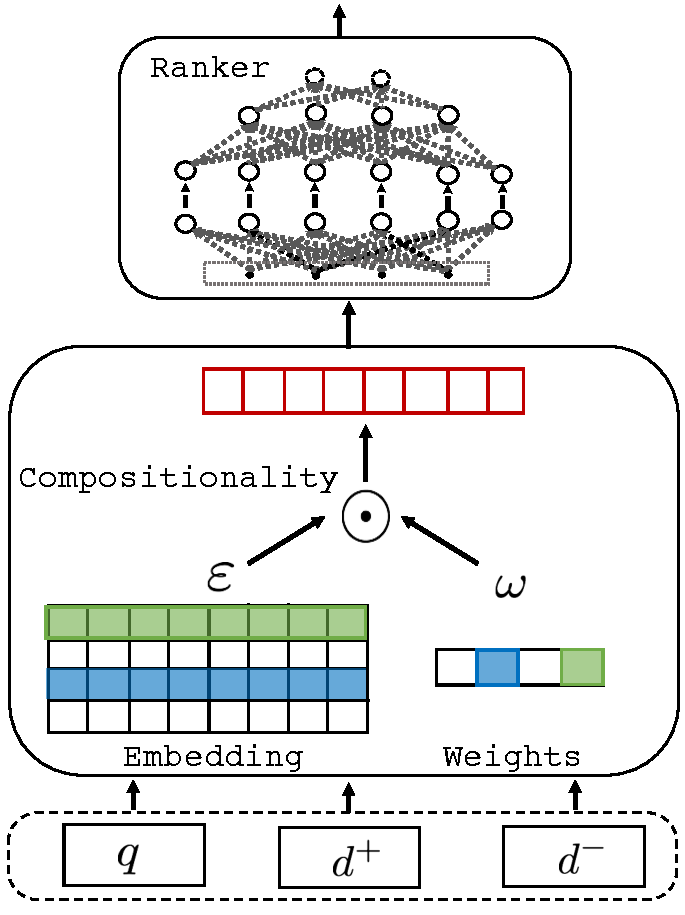
\includegraphics[width=0.35\textwidth]{03-part-02/chapter-05/figs_and_tables/fig_ranker.pdf}
    \caption{The document ranker used as \tch in \cws and \std in \fwl.}
    \label{fig:ranker}
\end{figure}


\subsubsection{The \tnet in \cws and the \std in \fwl}
We employ the pairwise neural ranker architecture explained in Section~\ref{sec:modeltwo} as the \tnet in \cws and \std in \fwl. 

Each training instance $x$ consists of a query $q$, and two documents $d^+$ and $d^-$. The labels, $\tilde{y}$ and $y$, are scalar values indicating the probability of $d^+$ being ranked higher than $d^-$ with respect to $q$.

\mypar{The Representation Learning Layer.}
This layer learns a function $\varepsilon: \mathcal{V} \rightarrow \mathbb{R}^{m}$  (where $\mathcal{V}$ denotes the vocabulary set, and $m$ is the number of embedding dimensions) that maps each word to its embedding which is downstream of the ranking task as well as a weighting function $\omega: \mathcal{V} \rightarrow \mathbb{R}$ which learns the global importance of each word. Then, the learned weights are used to compose word embeddings to generate query/document embeddings. The output of this layer is the concatenation of vectors representing query and two documents.
%
In our experiments, we initialize the embedding function $\varepsilon$ with word2vec embeddings~\cite{Mikolov:2013} pre-trained on Google News and the weighting function $\omega$ with IDF.

\mypar{The Supervision Layer.} 
This layer receives the vector representation of the inputs processed by the representation learning layer and outputs a prediction $\hat{y}_i$.
We opt for a simple fully connected feed-forward network with $l$ hidden layers followed by a sigmoid. We employ the weighted cross entropy loss:
\begin{equation}
% \nonumber
\small
\mathcal{L}_t = \sum_{i\in B_U} \tilde{c}_i [- \tilde{y}_i \log (\hat{y}_i) - (1-\tilde{y}_i) \log(1-\hat{y}_i)],
\end{equation}
where $B_U$ is a batch of instances from $U$, and $\tilde{c}_i$ is the confidence score of the weakly annotated instance $i$, estimated by the \cnet.

The general schema of the \tnet (or \std) is illustrated in Figure~\ref{fig:ranker}. More details are provided in Section~\ref{sec:modeltwo}.

\subsubsection{The \wa}
The \wa in the document ranking task is BM25~\citep{Robertson:2009}, a well-known unsupervised retrieval method. This method heuristically scores a given pair of query-document based on the statistics of their matched terms. In the pairwise document ranking setup, $\tilde{y}_i$ for a given sample $x_j = (q,d^+,d^-)$ is the probability of document $d^+$ being ranked higher than $d^-$: 
$\tilde{y}_i = P_{q,d^+,d^-} = \nicefrac{s_{q,d^+}}{s_{q,d^+} + s_{q,d^-}}$,  where $s_{q,d}$ is the score obtained from the \wa.


\subsubsection{The \cnet in \cws}
The \cnet is a regresses and we use a simple fully connected feed-forward network. To train the \cnet, the target label $c_j$ is calculated using the absolute difference of the strong label and the weak label: $c_j= 1-|y_j - \tilde{y}_j|$, where $y_j$ is calculated similar to $\tilde{y}_i$, but $s_{q,d}$ comes from strong labels provided by humans.


\subsubsection{The \tch in \fwl}
We use Gaussian Process as the \tch in order to generate soft labels. We pass the mean of $\mathcal{GP}$ through the same function $g(.)$ that is applied on the output of the \std network, where the $g(.)$ is sigmoid for the document ranking task.
Since we have one dimensional regression here, $\Sigma(x_t)$ is scalar and $h(.)$ is identity.
In the \tch, linear combinations of different kernels are used. For the document ranking task, we use sparse variational GP regression\footnote{\url{http://gpflow.readthedocs.io/en/latest/notebooks/SGPR_notes.html}}~\citep{Titsias2009variational} with this kernel:
\begin{equation}
k(x_i,x_j)=k_{\rm Matern3/2}(x_i,x_j)+{k_{\rm Linear}}(x_i,x_j)+k_{\rm White}(x_i,x_j)
\end{equation}

where,
\begin{flalign*}
    \hspace{6em}
    &&k_{\rm Matern3/2}(x_i,x_j) &= \left(1+\frac{\sqrt{3}\Vert x_i-x_j\Vert}{l}\right)\exp{\left(-\frac{\sqrt{3}\Vert x_i-x_j\Vert}{l}\right)} & \\
    &&k_{\rm Linear}(x_i,x_j) &= \sigma_0^2+x_i.x_j & \\
    &&k_{\rm White}(x_i,x_j) &= constant\_value, \quad \forall x_1=x_2 \text{ and } 0 \text{ otherwise} & 
\end{flalign*}

We empirically found $l=1$ satisfying value for the length scale of Matern3/2 kernel.
We also set $\sigma_0 = 0$ to obtain a homogeneous linear kernel. 
The constant value of $K_{White}(.,.)$ determines the level of noise in the labels. This is different from the noise in weak labels. This term explains the fact that even in strong labels there might be a trace of noise due to the inaccuracy of human labelers. 

It's noteworthy that we used clustered $\mathcal{GP}$ algorithm, explained in Section~\ref{sec:CGP}, and set the number of clusters to $50$ for this task..  


\subsubsection{Collections}
We use two standard TREC collections for the task of ad-hoc retrieval: The first collection (\emph{Robust04}) consists of 500k news articles from different news agencies as a homogeneous collection. The second collection (\emph{ClueWeb}) is ClueWeb09 Category B, a large-scale web collection with over 50 million English documents, which is considered as a heterogeneous collection. Spam documents were filtered out using the Waterloo spam scorer~\footnote{\url{http://plg.uwaterloo.ca/~gvcormac/clueweb09spam/}}~\citep{Cormack:2011} with the default threshold $70\%$. 

\mypar{Data with strong labels.} 
We take query sets that contain human-labeled judgments: a set of 250 queries (TREC topics 301--450 and 601--700) for the Robust04 collection and a set of 200 queries (topics 1-200) for the experiments on the ClueWeb collection.
For each query, we take all documents judged as relevant plus the same number of documents judged as non-relevant and form pairwise combinations among them.

\mypar{Data with weak labels.}
We create a query set $Q$ using the unique queries appearing in the AOL query logs~\citep{Pass:2006}. 
This query set contains web queries initiated by real users in the AOL search engine that were sampled from a three-month period from March 2006 to May 2006. 
We applied standard pre-processing~\cite{Dehghani:2017:SIGIR,Dehghani2017:CIKM} on the queries: We filtered out a large volume of navigational queries containing URL substrings (``http'', ``www.'', ``.com'', ``.net'', ``.org'', ``.edu''). We also removed all non-alphanumeric characters from the queries. For each dataset, we took queries that have at least ten hits in the target corpus using our \wa method. Applying all these steps, 
We collect 6.15 million queries to train on in Robust04 and 6.87 million queries for ClueWeb.
To prepare the weakly labeled training set $\mathcal{D}_w$, we take the top $1,000$ retrieved documents using BM25 for each query from training query set $Q$, which in total leads to $\sim|Q|\times 10^6$ training samples. 

\subsubsection{Experimental Setup.}
For the evaluation of the whole model, we conducted a 3-fold cross-validation. However, for each dataset, we first tuned all the hyper-parameters of the \tnet in \cws (and \std in the first step of \fwl) in the first step on the set with strong labels using batched GP bandits with an expected improvement acquisition function~\citep{Desautels:2014} and kept the optimal parameters of the \tnet (and \std) fixed for all the other experiments.
The size and number of hidden layers for the \tnet (and \std) is selected from $\{64, 128, 256, 512\}$. The initial learning rate and the dropout parameter were selected from $\{10^{-3}, 10^{-5}\}$ and $\{0.0, 0.2, 0.5\}$, respectively. We considered embedding sizes of $\{300, 500\}$. The batch size in our experiments was set to $128$.  We use ReLU~\citep{Nair:2010} as a non-linear activation function $\alpha$ in \tnet (and \std).  We use the Adam optimizer~\citep{Kingma:2014} for training, and \emph{dropout}~\citep{Srivastava:2014} as a regularization technique.

%
At inference time, for each query, we take the top $2,000$ retrieved documents using BM25 as candidate documents and re-rank them using the trained models. We use the Indri\footnote{\url{https://www.lemurproject.org/indri.php}} implementation of BM25 with default parameters (i.e., $k_1 = 1.2$, $b = 0.75$, and $k_3 = 1,000$).

\subsubsection{Results and Discussions} 
\label{sec:res_and_disc_ranking}
We conducted k-fold cross validation on $\mathcal{D}_s$ (the strong data) and report two standard evaluation metrics for ranking: mean average precision (MAP) of the top-ranked $1,000$
documents and normalized discounted cumulative gain calculated for the top $20$ retrieved documents (nDCG@20). 
Table~\ref{tbl_main} shows the performance on both datasets. As can be seen, \fwl and \cws both provide significant boost on the performance on top of the baseline methods over both datasets.


\begin{table}[tbp]
\renewcommand{\arraystretch}{1.1}
\caption{\label{tbl_main}Performance of \cws and \fwl as well as the main baseline methods, described in Table~\ref{tbl_baselines}, for the document ranking task. \pssmall{i} indicates that the improvements with respect to the baseline $i$ are statistically significant at the 0.05 level using the paired two-tailed t-test with Bonferroni correction.}
\centering
\begin{adjustbox}{max width=\textwidth}
\begin{tabular}{r l l l l l}
\toprule
& \multirow{2}{*}{Method} &
\multicolumn{2}{c}{Robust04} & \multicolumn{2}{c}{ClueWeb}
\\ 
\cmidrule(lr){3-4} \cmidrule(lr){5-6}
& & \small{MAP} & \small{nDCG@20}
& \small{MAP} & \small{nDCG@20}
\\ \midrule
1 & \small{WA$_\text{BM25}$} 
& 0.2503\pssmall{2} & 0.4102\pssmall{2}  
& 0.1021\pssmall{2} & 0.2070\pssmall{2}
\\ \midrule
2 & \small{$\text{NN}_{\text{S}}$} 
& 0.1790 & 0.3519  
& 0.0782 & 0.1730
\\
3 & \small{$\text{NN}_{\text{W}}$} 
& 0.2702\pssmall{12} & 0.4290\pssmall{12}  
& 0.1297\pssmall{12} & 0.2201\pssmall{12}
\\ \midrule
4 & \small{$\text{NN}_{\text{W}\text{/S}^+}$} 
&  0.2763\pssmall{123} & 0.4330\pssmall{123} 
&  0.1354\pssmall{123} & 0.2319\pssmall{123}
\\
5 & \small{$\text{NN}_{\text{W}} \to \text{NN}_{\text{S}}$} 
&  0.2810\pssmall{12346} & 0.4372\pssmall{12346} 
&  0.1346\pssmall{12346} & 0.2317\pssmall{12346}
\\
6 & \small{$\text{NN}_{\text{W}} \to \text{NN}^{\text{Sup}}_{\text{S}}$}
&  0.2711\pssmall{123} & 0.4203\pssmall{123} 
&  0.1002\pssmall{123} & 0.1940\pssmall{123}
\\
7 & \small{$\text{NN}_{\text{W}} \to \text{NN}^{\text{Rep}}_{\text{S}}$}
&  0.2810\pssmall{1234} & 0.4316\pssmall{1234} 
&  0.1286\pssmall{1234} & 0.2240\pssmall{1234}
\\
8 & \small{\cws}
&  0.3017\pssmall{1234567} & 0.4511\pssmall{1234567} 
&  0.1363\pssmall{1234567} & 0.2444\pssmall{1234567}
\\
13 & \small{\fwl}
& \textbf{0.3124}\pssmall{1234567}  & \textbf{0.460}\pssmall{1234567} & \textbf{0.1472}\pssmall{1234567}  & \textbf{0.2453}\pssmall{1234567}
\\\bottomrule
\end{tabular}
\end{adjustbox}
\end{table}



In the ranking task, the \std is designed in particular to be trained on weak annotations~\citep{Dehghani:2017:SIGIR}, hence training the network only on weak supervision, i.e. $\text{NN}_{\text{W}}$ performs better than $\text{NN}_{\text{S}}$. This can be due to the fact that ranking is a complex task requiring many training samples to learn representations that can be used to assess the relevance, while relatively few data with strong labels are available.

Alternating between strong and weak data during training, i.e. $\text{NN}_{\text{W}\text{/S}^+}$ seems to bring little (but statistically significant) improvement. However, we can gain better results by the typical fine-tuning strategies.  Among the fine-tuning experiments, updating all the parameters of the \tnet (or \std), i.e. $\text{NN}_{\text{W}} \to \text{NN}_{\text{S}}$, is the best fine-tuning strategy. Updating only the parameters of the representation layer based on the strong labels, i.e. $\text{NN}_{\text{W}} \to \text{NN}^{\text{Rep}}_{\text{S}}$, works better than updating only parameters of the supervision layer, i.e. $\text{NN}_{\text{W}} \to \text{NN}^{\text{Sup}}_{\text{S}}$. This supports our designed choice of a shared embedding layer in \cws which gets updated on set $V$.

\fwl is the best performing baselines, and \cws achieves 97\% of the performance of \fwl. The main advantage of \cws over \fwl is that it is trained in a single stage process and needs to meet the examples in $\mathcal{D}_w$ (which is a reasonably large set) only one time, while \fwl has three sequential stages during training and it needs to iterate two times over all the examples in $\mathcal{D}_w$. Also employing a Gaussian Process as part of the model in \fwl limits its scalability, while the components of \cws are all neural networks, and this eases the increase in the capacity of the model. 
% With all that, we find \cws a much more efficient model in terms of training cost, with losing little to no performance.


\begin{table}[tbp]
% \renewcommand{\arraystretch}{1.1}
\caption{\label{tbl_variants_rank_cws}Performance of the variants of the \cws on different datasets for document ranking task. Baselines are described in Table~\ref{tbl_baselines}.}
\centering
\begin{adjustbox}{max width=\textwidth}
\begin{tabular}{r l c c c c}
\toprule
& \multirow{2}{*}{\textbf{Method}} &
\multicolumn{2}{c}{\textbf{Robust04}} & \multicolumn{2}{c}{\textbf{ClueWeb}}
\\ 
\cmidrule(lr){3-4} \cmidrule(lr){5-6}
& & \small{\textit{MAP}} & \small{\textit{nDCG@20}}
& \small{\textit{MAP}} & \small{\textit{nDCG@20}}
\\ \midrule
\bf 8 & \bf \small{\cws}
&  \textbf{0.3017} & \textbf{0.4511}
&  0.1363 & \textbf{0.2444}
\\
\bf 9 & \bf \small{CWS$_\text{JT}^+$} 
& 0.2786  & 0.4367  
& 0.1310  & 0.2244 
\\ 
\bf 10 & \bf \small{CWS$_\text{ST}$} 
&  0.2716  & 0.4237 
&  0.1320  & 0.2213
\\
\bf 11 & \bf \small{\cws$_\text{CT}$} 
&  0.2961 & 0.4440 
&  \textbf{0.1378}  & 0.2431 
\\ 
\bf 12 & \bf \small{\cws$_\text{PT}$} 
& 0.2784  & 0.4292  
& 0.1314  & 0.2207
\\\bottomrule
\end{tabular}
\end{adjustbox}
\end{table}


As an ablation study on \cws, we tried different training strategies and report the results in Table~\ref{tbl_variants_rank_cws}. As shown, \cws and CWS$_\text{CT}$ perform better than other strategies.
%
\cws$_\text{CT}$ is to let the \cnet to be trained separately, while still being able to enjoy shared learned information from the \tnet. Compared to \cws, \cws$_\text{CT}$ is less efficient as we need two rounds of training on weakly labeled data. 

While it seems reasonable to make use of strong labels for updating \emph{all} parameters of the \tnet, CWS$_\text{JT}^+$ achieves no better results than \cws. We speculate that during training, the direction of the parameter optimization is profoundly affected by the type of supervision signal and while we control the magnitude of the gradients, we do not change their directions. Hence alternating between two sets with different label qualities (different supervision signal types, i.e. weak and strong) confuses the supervision layer of the \tnet. 

In \cws$_\text{ST}$,  the strong dataset, $\mathcal{D}_s$, is too small to train a high-quality \cnet without taking advantage of the vast amount of weakly annotated data in $\mathcal{D}_w$ to learn better representations, so CWS$_\text{ST}$ is not able to improve the performance over $\text{NN}_W$ significantly and also we noticed that this strategy leads to a slow convergence compared to the $\text{NN}_W$. 
Also transferring learned information from \tnet to \cnet via progressive training, i.e., CWS$_\text{PT}$, performs no better than full sharing of the representation learning layer.



\begin{table}[tbp]
% \renewcommand{\arraystretch}{1.1}
\caption{\label{tbl_variants_rank_fwl}Performance of \fwl against some of the baselines on different datasets for document ranking task. Baselines are described in Table~\ref{tbl_baselines}.}
\centering
\begin{adjustbox}{max width=\textwidth}
\begin{tabular}{r l c c c c}
\toprule
& \multirow{2}{*}{\textbf{Method}} &
\multicolumn{2}{c}{\textbf{Robust04}} & \multicolumn{2}{c}{\textbf{ClueWeb}}
\\ 
\cmidrule(lr){3-4} \cmidrule(lr){5-6}
& & \small{\textit{MAP}} & \bf \small{\textit{nDCG@20}}
&  \small{\textit{MAP}} & \bf \small{\textit{nDCG@20}}
\\ \midrule
\bf 13 & \bf \small{\fwl}
& \textbf{0.3124}  & \textbf{0.4607}
& \textbf{0.1472} & \textbf{0.2453}
\\
\bf 14 & \bf  \small{$\text{NN}_{\text{W}^\omega \to \text{NN}_\text{S}}$}
&  0.2899 & 0.4431
&  0.1320 & 0.2309
\\ 
\bf 15 & \bf \small{\fwlnospace$_{unsuprep}$} 
&  0.2211 & 0.3700
&  0.0831 & 0.1964
\\
\bf 16 & \bf \small{\fwlnospace$\backslash\Sigma$} 
&  0.2980 & 0.4516
&  0.1386 & 0.2340
\\\bottomrule
\end{tabular}
\end{adjustbox}
\end{table}
Table~\ref{tbl_variants_rank_fwl} presents the results of some experiments we have done as ablation studies on \fwl. 

Weighting the gradient updates from weak labels during pretraining and fine-tuning the network with strong labels, i.e. NN$_{\text{W}^\omega \to \text{S}}$ seems to work quite well.
%
Comparing the performance of \fwlnospace$_{unsuprep}$ to \fwl indicates that, first of all learning the representation of the input data downstream of the main task leads to better results compared to a task-independent unsupervised or self-supervised way. Also the dramatic drop in the performance compared to the \fwl, emphasizes the importance of the preretraining the \std on weakly labeled data.

%
We can gain improvement by fine-tuning the NN$_\text{W}$ using labels generated by the \tch without considering their confidence score, i.e. \fwl$\backslash\Sigma$. This means we just augmented the fine-tuning process by generating a fine-tuning set using \tch which is better than $\mathcal{D}_s$ in terms of quantity and $\mathcal{D}_w$ in terms of quality. This baseline is equivalent to setting $\beta = 0$ in Equation~\ref{eqn:eta2}. However, we see a big jump in performance when we use \fwl to include the estimated label quality from the \tch, leading to the best overall results.

\subsection{Sentiment Classification}
In sentiment classification, the goal is to predict the sentiment (e.g., positive, negative, or neutral) of a sentence. Each training sample $x$ consists of a sentence $s$ and its sentiment label $\tilde{y}$.

\begin{figure}[t!]
    \centering
            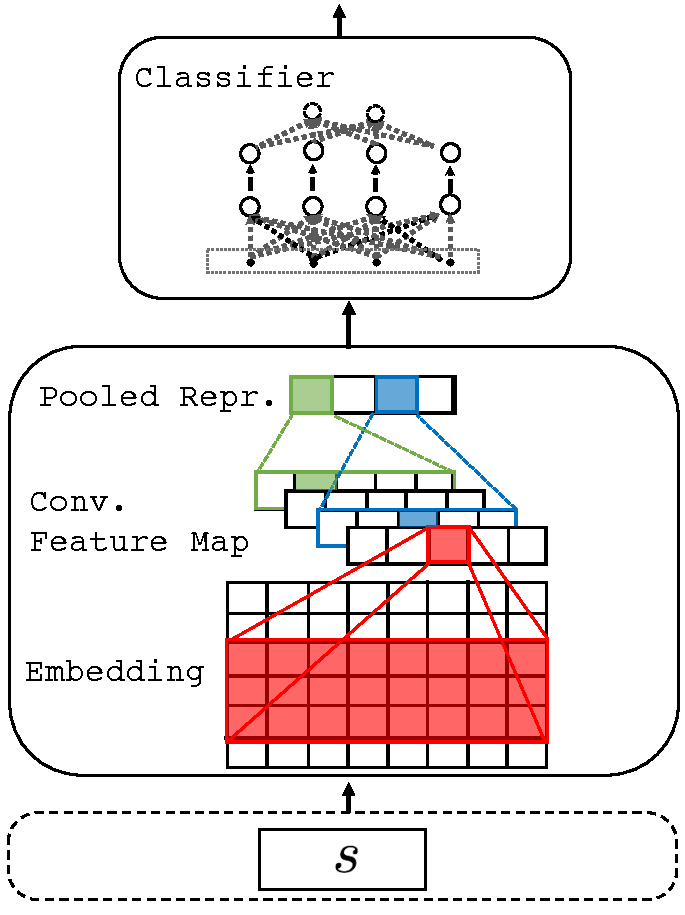
\includegraphics[width=0.35\textwidth]{03-part-02/chapter-05/figs_and_tables/fig_sentiment.pdf}
    \caption{The sentiment classifier used as \tch in \cws and \std in \fwl.}
    \label{fig:sentiment}
\end{figure}


\subsubsection{The \tnet in \cws and the \std in \fwl}
We use a convolutional model~\citep{Kim:2014} as the \tnet in \cws and the \std in \fwl, which is similar to the state-of-the-art model for Twitter sentiment classification from Semeval 2015 and 2016~\cite{Severyn:2015:SemEval,Deriu2016:SemEval,Deriu:2017,Severyn:2015:SIGIR}.

\mypar{The Representation Learning Layer} 
The representation learning layer in this task consists of an embedding function $\varepsilon: \mathcal{V} \rightarrow \mathbb{R}^{m}$, where $\mathcal{V}$ denotes the vocabulary set and $m$ is the number of embedding dimensions.

This function maps the sentence to a matrix $S \in \mathbb{R}^{m \times |s|}$, where each column represents the embedding of a word at the corresponding position in the sentence. We initialize the embedding matrix with word2vec embeddings~\cite{Mikolov:2013} pretrained on a collection of 50M tweets.

Matrix $S$ is passed through a convolution layer.  In this layer, a set of $f$ filters is applied to a sliding window of length $h$ over $S$ to generate a feature map matrix $O$. Each feature map $o_i$ for a given filter $F$ is generated by $o_i = \sum_{k,j}S[i:i+h]_{k,j} F_{k,j}$, where $S[i:i+h]$ denotes the concatenation of word vectors from position $i$ to $i+h$. The concatenation of all $o_i$ produces a feature vector $o \in \mathbb{R}^{|s|-h+1}$. The vectors $o$ are then aggregated over all $f$ filters into a feature map matrix $O \in \mathbb{R}^{f\times(|s|-h+1)}$.

We also add a bias vector $b \in R^f$ to the result of a convolution.
Each convolutional layer is followed by a non-linear activation function (we use ReLU\cite{Nair:2010}) which is applied element-wise. Afterward, the output is passed to the max pooling layer which operates on columns of the feature map matrix $O$ returning the largest value: $pool(o_i) : \mathbb{R}^{1\times(|s|-h+1)} \rightarrow \mathbb{R}$.

\mypar{The Supervision Layer.} 
This layer is a simple fully connected feed-forward network with $l$ hidden layers, followed by a softmax.  We employ the weighted cross entropy loss:
\begin{equation}
% \nonumber
\mathcal{L}_t = \sum_{i\in B_U} \tilde{c}_i \sum_{k \in K} - \tilde{y}_i^k \log (\hat{y}_i^k),
\end{equation}
where $B_U$ is a batch of instances from $U$, and $\tilde{c}_i$ is the confidence score of the weakly annotated instance $i$, and $K$ is a set of classes. 
The general schema of the \tnet (or \std) is illustrated in Figure~\ref{fig:sentiment}.

\subsubsection{The \wa}
\label{sentiment-WA}
The \wa for the sentiment classification task is a simple lexicon-based method~\citep{Hamdan:2013,Kiritchenko:2014}.
We use SentiWordNet03~\citep{Gaccianella:2010} to assign probabilities (positive, negative and neutral) for each token in set $\mathcal{D}_w$. We use a bag-of-words model for the sentence-level probabilities (i.e.\ just averaging the distributions of the terms), yielding a noisy label $\tilde{y}_i \in \mathbb{R}^{|K|}$, where $|K|=3$ is the number of classes.  We found empirically that using soft labels from the \wa works better than assigning a single hard label.


\subsubsection{The \cnet in \cws}
In this task, the \cnet is also a regresses and we use a simple fully connected feed-forward network. The target label $c_j$ for the \cnet is calculated by using the mean absolute difference of the strong label and the weak label: $c_j= 1-\frac{1}{|K|}\sum_{k\in K}|y_j^k - \tilde{y}_j^k|$, where $y_j$ is the one-hot encoding of the sentence label over all classes.


\subsubsection{The \tch in \fwl}
Similar to the ranking task, we use Gaussian Process as the \tch in order to generate soft labels. We pass the mean of $\mathcal{GP}$ through the same function $g(.)$ that is applied on the output of the \std network, where the $g(.)$ is softmax for the sentiment classification task.
Here in this task, $h(.)$ is an aggregation function that takes variance over several dimensions and outputs a single measure of variance. As a reasonable choice, the aggregating function $h(.)$ in the sentiment classification task (three classes) is \emph{mean} of variances over dimensions. 
In the \tch, linear combinations of different kernels are used. For the sentiment classification task, We use sparse variational GP for multiclass classification\footnote{\url{http://gpflow.readthedocs.io/en/latest/notebooks/multiclass.html}}~\citep{hensman2014scalable} with the following kernel:
\begin{equation}
k(x_i,x_j)=k_{\rm RBF}(x_i,x_j)+{k_{\rm Linear}}(x_i,x_j)+k_{\rm White}(x_i,x_j)
\end{equation}
where,
\begin{flalign*}
    \hspace{6em}
    &&k_{\rm RBF}(x_i,x_j) &= \exp{\left(\frac{\Vert x_i-x_j\Vert^2}{2l^2}\right)} & 
    \\
    &&k_{\rm Linear}(x_i,x_j) &= \sigma_0^2+x_i.x_j & \\
    &&k_{\rm White}(x_i,x_j) &= constant\_value, \quad \forall x_1=x_2 \text{ and } 0 \text{ otherwise} & 
\end{flalign*}

Similar to the ranking task, we set $l=1$ the length scale of RBF kernel, set $\sigma_0 = 0$  for the linear kernel, and set the number of clusters to $30$ in clustered $\mathcal{GP}$ algorithm.


\subsubsection{Collections}
We test our model on the twitter message-level sentiment classification of SemEval-15 Task 10B \citep{rosenthal:2015}. Datasets of SemEval-15 subsume the test sets from previous editions of SemEval, i.e. SemEval-13 and SemEval-14. Each tweet was preprocessed so that URLs and usernames are masked.

\mypar{Data with strong labels.} 
We use train (9,728 tweets) and development (1,654 tweets) data from SemEval-13 for training and SemEval-13-test (3,813 tweets) for validation.
To make your results comparable to the official runs on SemEval we us SemEval-14 (1,853 tweets) and  SemEval-15 (2,390 tweets) as test sets~\citep{rosenthal:2015, Nakov:2016}.

\mypar{Data with weak labels.}
We use a large corpus containing 50M tweets collected during two months for both, training the word embeddings and creating the weakly annotated set $\mathcal{D}_w$ using the lexicon-based method explained in Section~\ref{sentiment-WA}. 

\subsubsection{Experimental Setup.}
Similar to the document ranking task, we tuned hyper-parameters for the \tnet in \cws (and \std in the first step of \fwl) with respect to the strong labels of the validation set using batched GP bandits with an expected improvement acquisition function~\citep{Desautels:2014} and kept the optimal parameters fixed for all the other experiments.  
The size and number of hidden layers for the classifier and is selected from $\{32, 64, 128\}$.
We tested the model with both, $1$ and $2$ convolutional layers. The number of convolutional feature maps and the filter width is selected from $\{200,300\}$ and $\{ 3, 4, 5\}$, respectively. The initial learning rate and the dropout parameter were selected from $\{1E-3, 1E-5\}$ and $\{0.0, 0.2, 0.5\}$, respectively. We considered embedding sizes of $\{100, 200\}$ and the batch size in these experiments was set to $64$. ReLU~\citep{Nair:2010} is used as a non-linear activation function in \tnet (and \std).  Adam optimizer~\citep{Kingma:2014} is used for training, and \emph{dropout}~\citep{Srivastava:2014} as a regularizer.

In the rest of the chapter, we will present the main results of the introduced baseline methods and the proposed models, \cws and \fwl, 


\subsubsection{Results and Discussions} 
\begin{table}[!t]
            \renewcommand{\arraystretch}{1.1}
            \centering
            \caption{\label{tbl_main_sent}Performance ofof \cws and \fwl as well as the main baseline methods,described in Table~\ref{tbl_baselines}, for the sentiment classification task. 
            \pssmall{i} indicates that the improvements with respect to the baseline $i$ are statistically significant at the 0.05 level using the paired two-tailed t-test with Bonferroni correction.}
            \begin{tabular}{r l l l}
            \toprule
            & \textbf{Method} & \textbf{SemEval-14} & \textbf{SemEval-15}
            \\ \midrule
            \bf 1 & \bf \small{WA$_\text{Lexicon}$} 
            & 0.5141 & 0.4471
            \\ \midrule
           \bf  2 & \bf \small{$\text{NN}_{\text{S}}$} 
            & 0.6307\pssmall{1} & 0.5811\pssmall{13}
            \\
            \bf 3 & \bf \small{$\text{NN}_{\text{W}}$} 
            & 0.6719\pssmall{12} & 0.5606\pssmall{1} 
            \\ \midrule
            \bf 4 & \bf \small{$\text{NN}_{\text{W}\text{/S}^+}$} 
            & 0.7032\pssmall{12367} & 0.6319\pssmall{12367}
            \\
            \bf 5 & \bf \small{$\text{NN}_{\text{W}} \to \text{NN}_{\text{S}}$}
            & 0.7080\pssmall{12367} & 0.6441\pssmall{12367}
            \\
           \bf  6 & \bf \small{$\text{NN}_{\text{W}} \to \text{NN}^{\text{Sup}}_{\text{S}}$} 
            & 0.6875\pssmall{123} & 0.6193\pssmall{123}
            \\
            \bf 7 & \bf \small{$\text{NN}_{\text{W}} \to \text{NN}^{\text{Rep}}_{\text{S}}$}
            & 0.6932 \pssmall{123} & 0.6102\pssmall{123}
            \\ \midrule
            \bf 8 & \bf \small{\cws} 
            & 0.7362 \pssmall{1234567} & 0.6626\pssmall{1234567}
            \\
            \bf 13 & \bf \small{\fwl} 
            & \textbf{0.7470} \pssmall{12345678} & \textbf{0.6830}\pssmall{12345678}
            \\ \midrule
            \bf $\ast$ & \bf \small{SemEval$^\text{Best}$} 
            & 0.7162~\citep{Rouvier:2016} & 0.6618~\citep{Deriu2016:SemEval}
            \\\bottomrule
            \end{tabular}
\end{table}
We report Macro-F1, the official SemEval metric, in Table~\ref{tbl_main_sent}. 

Among all the baselines, \fwl is the best performing approach. \cws is also outperforms all the baselines. 

For this task, since the amount of data with strong labels are larger compared to the ranking task, the performance of $\text{NN}_{\text{S}}$ is acceptable. Alternately sampling from weak and strong data, i.e.  $\text{NN}_{\text{W}\text{/S}^+}$ gives better results than either of learning from just weak or just strong labels. However, pretraining on weak labels then fine-tuning both the supervision layer and the representation learning layer on strong labels, further improves the performance.  

Besides the baselines, we also report the best performing systems which are also convolution-based models (\citealt{Rouvier:2016} on SemEval-14; \citealt{Deriu2016:SemEval} on SemEval-15). Both \cws and \fwl outperform these methods.


\begin{table}[!t]
            \renewcommand{\arraystretch}{1.1}
            \centering
            \caption{\label{tbl_variants_sent_cws}Performance of the variants of the \cws on different datasets for the sentiment classification task. Baselines are described in Table~\ref{tbl_baselines}.}
            \begin{tabular}{r l l l}
            \toprule
            & Method & SemEval-14 & SemEval-15
            \\ \midrule
            8 & \small{\cws} 
            & 0.7362 & 0.6626
            \\
            9 & \small{\cws$_\text{JT+}$} 
            & 0.7310 & 0.6551
            \\
            10 & \small{\cws$_\text{ST}$} 
            & 0.7183 & 0.6501
            \\
            11 & \small{\cws$_\text{CT}$} 
            & \textbf{0.7363} & \textbf{0.6667}
            \\
            12 & \small{\cws$_\text{PT}$}
            & 0.7009 & 0.6118
            \\\bottomrule
            \end{tabular}
\end{table}
Similar to the ranking task, we have done an ablation study on \cws by trying different strategies for training \cws. The results of these experiments are presented in Table~\ref{tbl_variants_sent_cws}. \cws$_\text{CT}$ archives the highest performance among all the training strategies, however, as we discussed in Section~\ref{sec:res_and_disc_ranking}, it is not as efficient as \cws. 

In sentiment classification, compared to the ranking task, it is easier to estimate the confidence score of instances concerning the amount of available supervised data. Therefore, \cws$_\text{ST}$ improves the performance over $\text{NN}_{\text{S}}$ in Table~\ref{tbl_main_sent}. 


\begin{table}[!t]
            \renewcommand{\arraystretch}{1.1}
            \centering
            \caption{\label{tbl_variants_sent_fwl}Performance of \fwl against some of the baselines on different datasets for document ranking task. Baselines are described in Table~\ref{tbl_baselines}.}
            \begin{tabular}{r l c c}
            \toprule
            & \textbf{Method} & \textbf{SemEval-14} & \textbf{SemEval-15}
            \\ \midrule
            \bf 13 & \bf \small{\fwl} 
            & \textbf{0.7470} & \textbf{0.6830}
            \\
            \bf 14 & \bf \small{$\text{NN}_{\text{W}^\omega \to \text{NN}_\text{S}}$} 
            & 0.7166 & 0.6603
            \\
            \bf 15 & \bf \small{\fwlnospace$_{unsuprep}$} 
            & 0.6588  & 0.6954
            \\ 
            \bf 16 & \bf \small{\fwlnospace$\backslash\Sigma$} 
            & 0.7202 & 0.6590
            \\\bottomrule
            \end{tabular}
\end{table}
The results of a set of experiments we have done as ablation studies on \fwl is presented Table~\ref{tbl_variants_sent_fwl}. 

Having static weighting on the gradient updates, i.e. NN$_{\text{W}^\omega \to \text{S}}$, leads to the performance that is better than simple fine-tuning, i.e. $\text{NN}_{\text{W}} \to \text{NN}_{\text{S}}$ in Table~\ref{tbl_main_sent} .
%
For this task, similar to the ranking task, learning the representation in an unsupervised task independent fashion, i.e. \fwlnospace$_{unsuprep}$, does not lead to good results compared to the \fwl.
%
Similar to the ranking task, fine-tuning $\text{NN}_{\text{W}}$ based on labels generated by $\mathcal{GP}$ instead of data with strong labels, regardless of the confidence score, i.e. \fwl$\backslash\Sigma$, works better than standard fine-tuning. 

\section{Discussion and Analysis}
\label{sec:discussion}
\shrink
In this section, we provide further analysis by investigating the learning pace in \cws and \fwl, bias-variance trade-off in \fwl, sensitivity of \fwl to the quality of weak labels, and how modifying the learning rate in \fwl can be different from weighted sampling of training examples.

\subsection{Faster Learning Pace in \cws}
\label{sec:learning_pace}
\begin{figure}[!t]%
    \centering
    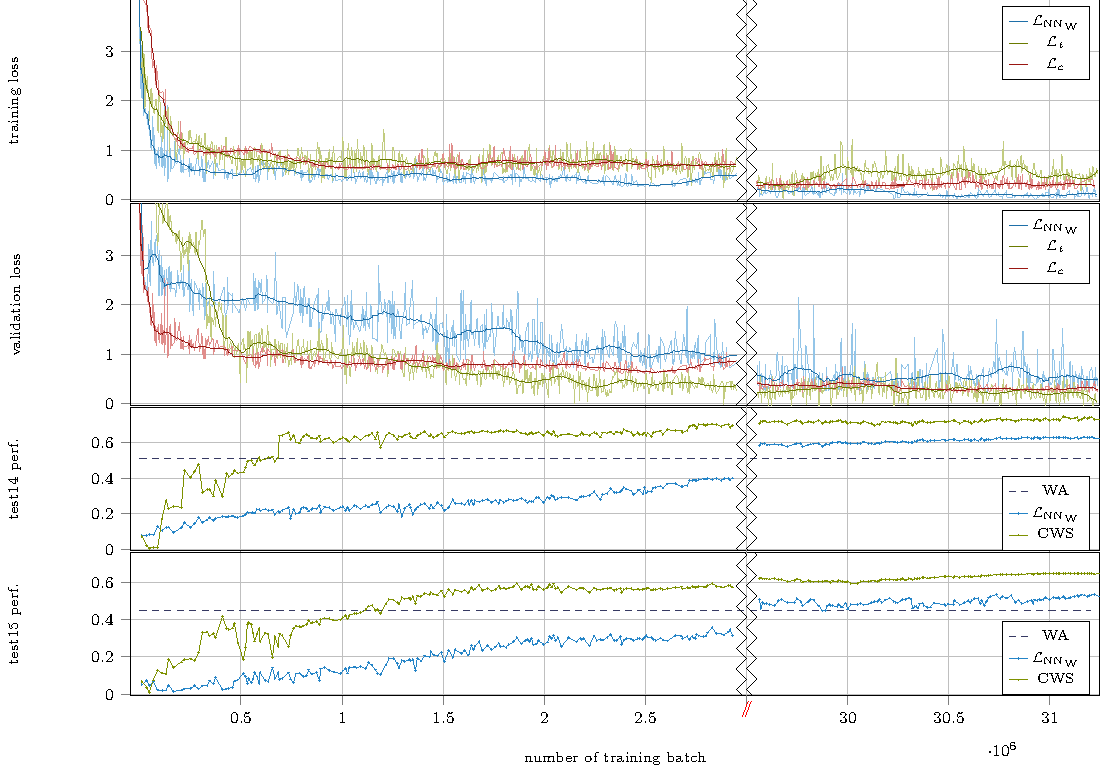
\includegraphics[width=0.8\textwidth]{03-part-02/chapter-05/figs_and_tables/plot_loss_cws.pdf}
    \caption{Loss of the \tnet ($\mathcal{L}_t$) and the \cnet ($\mathcal{L}_c$) compared to the loss of $\text{NN}_{\text{W}}$ ($\mathcal{L}_{\text{NN}_{\text{W}}}$) on training/validation set and performance of \cws, $\text{NN}_{\text{W}}$, and \wa on test sets with respect to different amount of training data on sentiment classification.}
    \label{fig:plot_loss_cws}
\end{figure}
In \cws, controlling the contribution of the weak labels on updating the parameters of the model not only improves the performance, but also provides the network with more solid signals which speeds up the learning process. 

Figure~\ref{fig:plot_loss_cws} illustrates the training/validation loss for both networks compared to the loss of training the \tnet with weak supervision, along with their performance on test sets, with respect to different amounts of training data for the sentiment classification task.
As shown, in training, the loss of the \tnet in our model, i.e., $\mathcal{L}_t$ is higher than the loss of the network which is trained only on weakly supervised data, i.e., $\mathcal{L}_{\text{NN}_{\text{W}}}$. 
%
However, since these losses are calculated with respect to the weak labels (not true labels), having very low training loss can be an indication of overfitting to the imperfection in the weak labels. 
%
In other words, regardless of the general problem of lack of generalization due to overfitting, in the setup of learning from weak labels, predicting labels that are similar to train labels (very low training loss) is not necessarily a desirable incident. 

In the validation set, however, $\mathcal{L}_t$ decreases faster than $\mathcal{L}_{\text{NN}_{\text{W}}}$, which supports the fact that $\mathcal{L}_{\text{NN}_{\text{W}}}$ overfits to the imperfection of weak labels, while our setup helps the \tnet to escape from this imperfection and do an excellent job on the validation set.
%
In terms of the performance, compared to $\text{NN}_{\text{W}}$, the performance of CWS on both test sets increases very quickly and CWS can pass the performance of the \wa by seeing much fewer instances annotated by the \wa.
\subsection{A Good Teacher is Better Than Many Observations} 

We also look at the rate of learning for the \std in \fwl as the amount of training data is varied. We performed two types of experiments for all tasks:
%
\begin{itemize}
    \item In the first experiment, we use all the available strong data but consider different percentages of the entire weak dataset.
    \item In the second experiment, we fix the amount of weak data and provide the model with varying amounts of strong data.
\end{itemize} 
We use standard fine-tuning with similar setups as for the baseline models. 
We fixed everything in the model and tried running the fine-tuning step with different values for $\beta \in \{0.0, 0.1, 1.0, 2.0, 5.0\}$ in all the experiments.
For the experiments on toy problem in Section~\ref{sec:learning_pace}, the reported numbers are averaged over 10 trials. In the first experiment (i.e. Figure~\ref{fig:plot_dw}), the size of sampled data data is: $|\mathcal{D}_s| = 50$ and $|\mathcal{D}_w| = 100$ (Fixed) and for the second one (i.e. Figure~\ref{fig:plot_dw}): $|\mathcal{D}_w| = 100$ and $|\mathcal{D}_s| = 10$ (fixed). 

Figure~\ref{fig:learning_rate} presents the results of these experiments. In general, for all tasks and both setups, the \std learns faster when there is a \tch.
One caveat is in the case where we have a very small amount of weak data. In this case the \std cannot learn a suitable representation in the first step, and hence the performance of \fwl is pretty low, as expected. It is highly unlikely that this situation occurs in reality as obtaining weakly labeled data is much easier than strong data.

The empirical observation of Figure~\ref{fig:learning_rate} that our model learns more with less data can also be seen as evidence in support of another perspective to \fwl, called \emph{learning using privileged information}~\citep{vapnik2015learning} which we explained in Section~\ref{sec:LUPI}. 
\begin{figure}[!t]%
    \centering
    \begin{subfigure}[t]{0.7\textwidth}
        \centering
        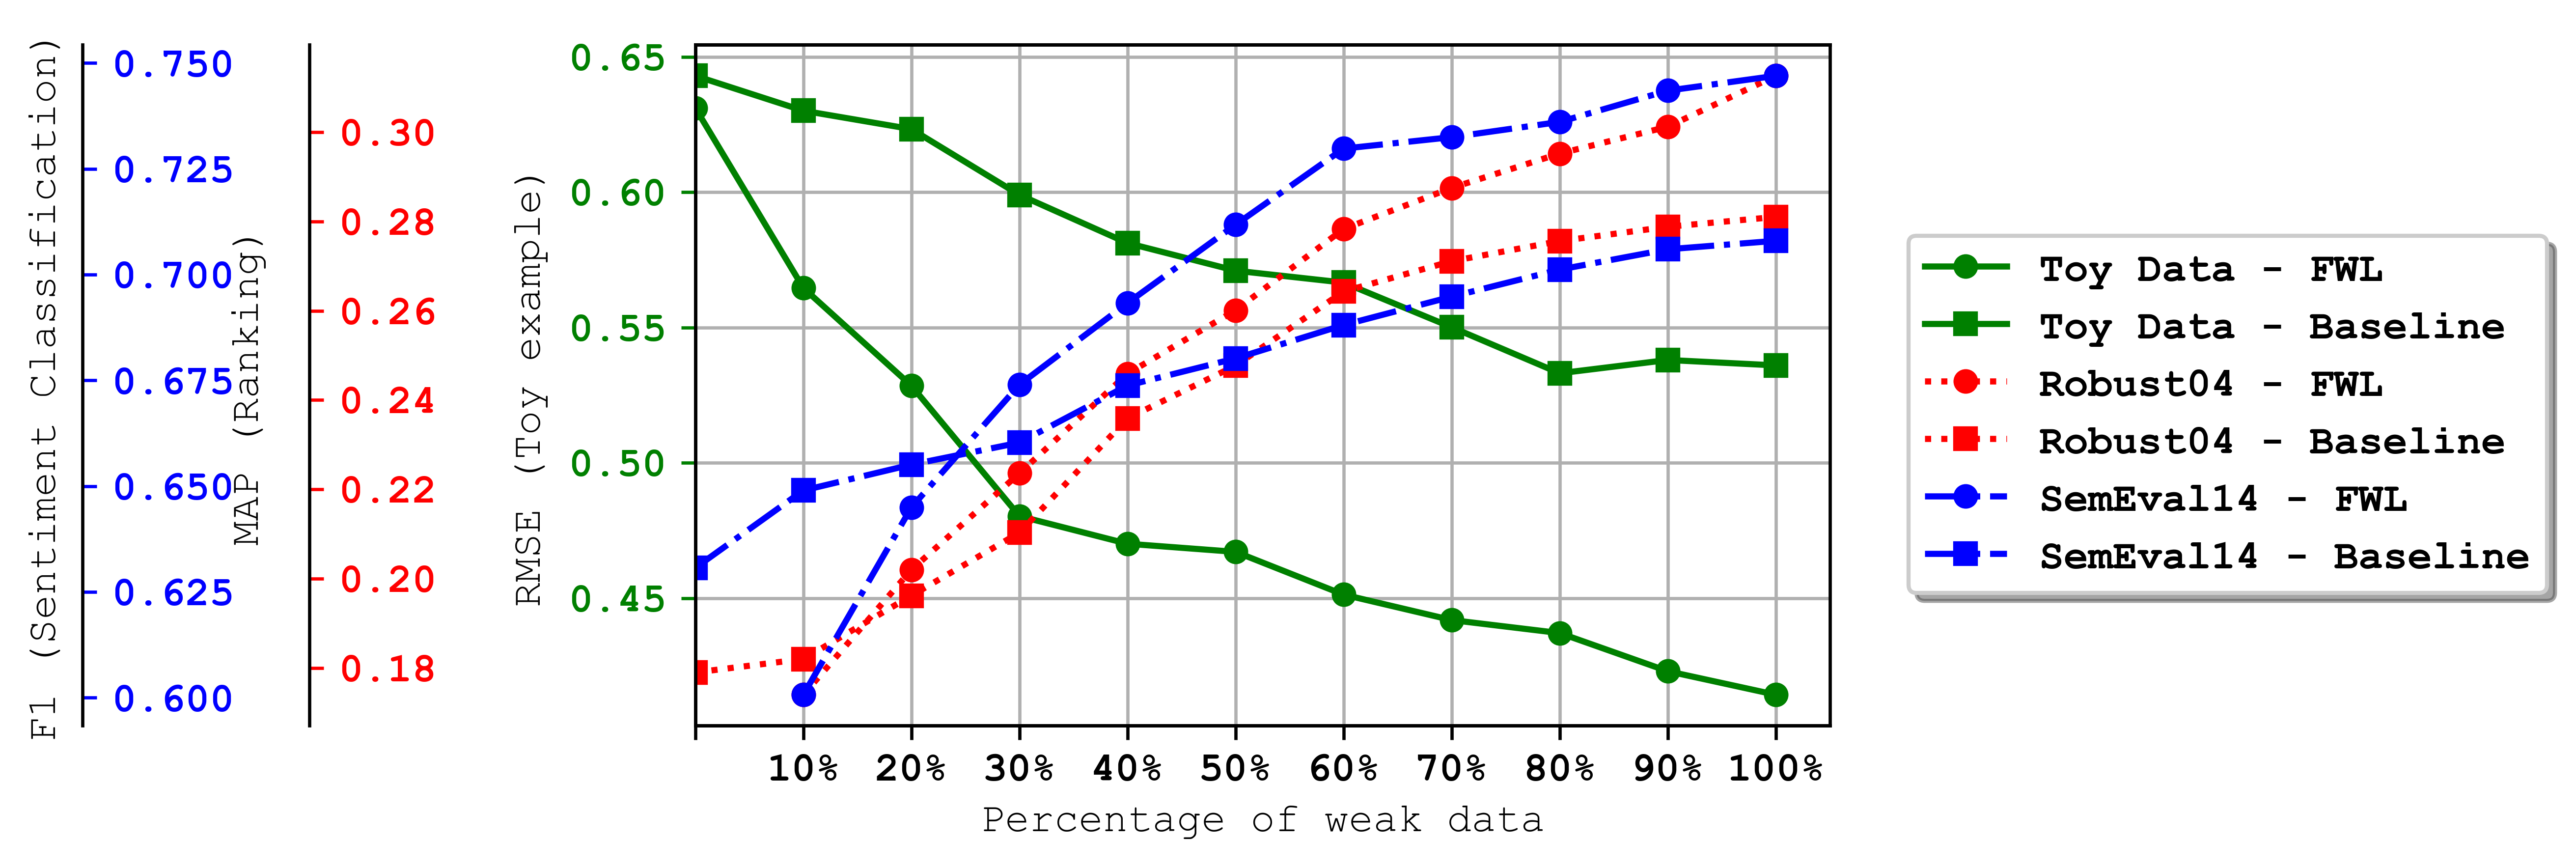
\includegraphics[width=\textwidth]{03-part-02/chapter-05/figs_and_tables/fig_data_w.png}
        \caption{\label{fig:plot_dw}\footnotesize{Models trained on different amount of weak data.}}
    \end{subfigure}%
    \hfill
    \begin{subfigure}[t]{0.7\textwidth}
        \centering
        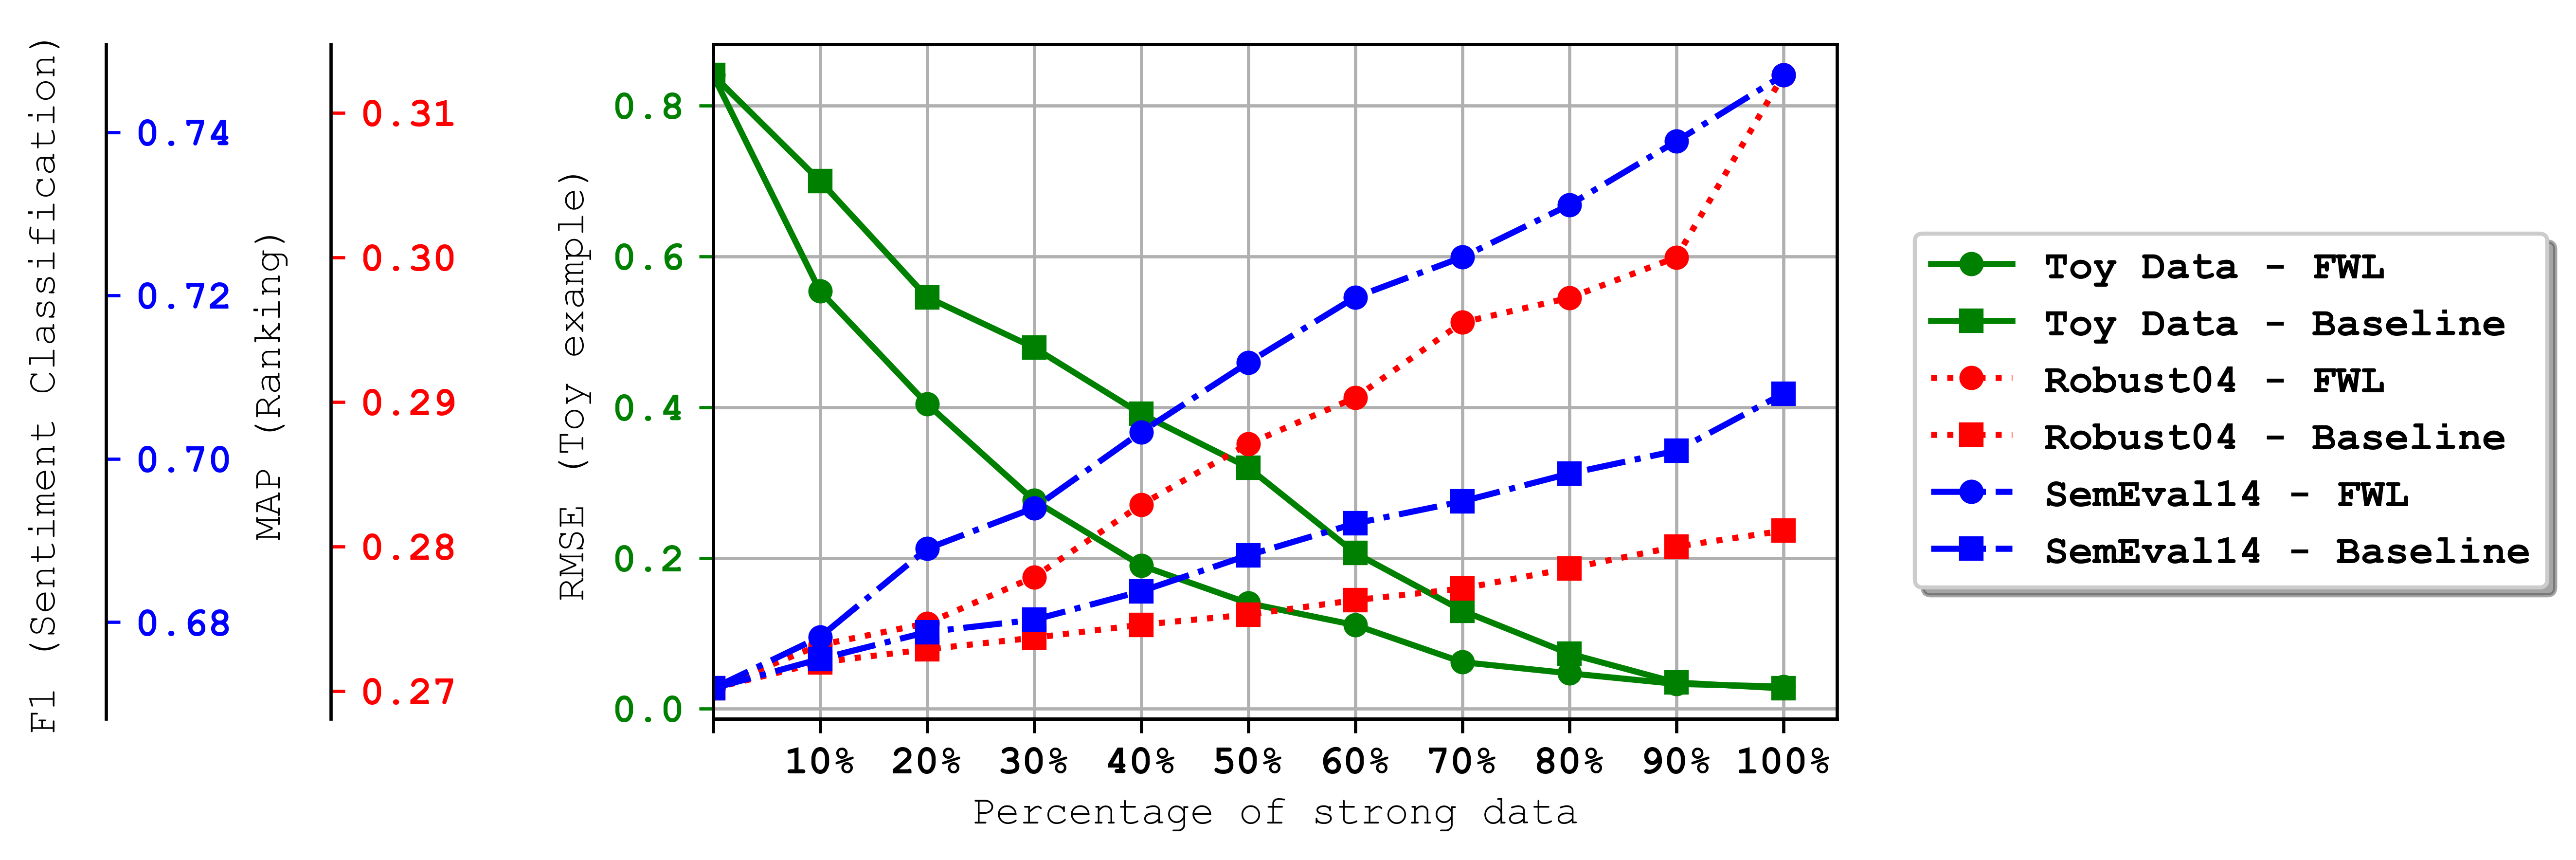
\includegraphics[width=\textwidth]{03-part-02/chapter-05/figs_and_tables/fig_data_s.png}
        \caption{\label{fig:plot_dt}\footnotesize{Models trained on different amount of strong data.}}
    \end{subfigure}%
    \caption{Performance of \fwl and the baseline model trained on different amount of data.}
    \label{fig:learning_rate}
\end{figure}


\subsection{Handling the Bias-Variance Trade-off in \fwl}
\label{sec:bias-variance}
As mentioned in Section~\ref{sec:proposed-method}, $\beta$ is a hyperparameter that controls the contribution of weak and strong data to the training procedure. In order to investigate its influence, we fixed everything in the model and ran the fine-tuning step with different values of $\beta \in \{0.0, 0.1, 1.0, 2.0, 5.0\}$ in all the experiments.

%
\begin{figure}[t]
    \centering
    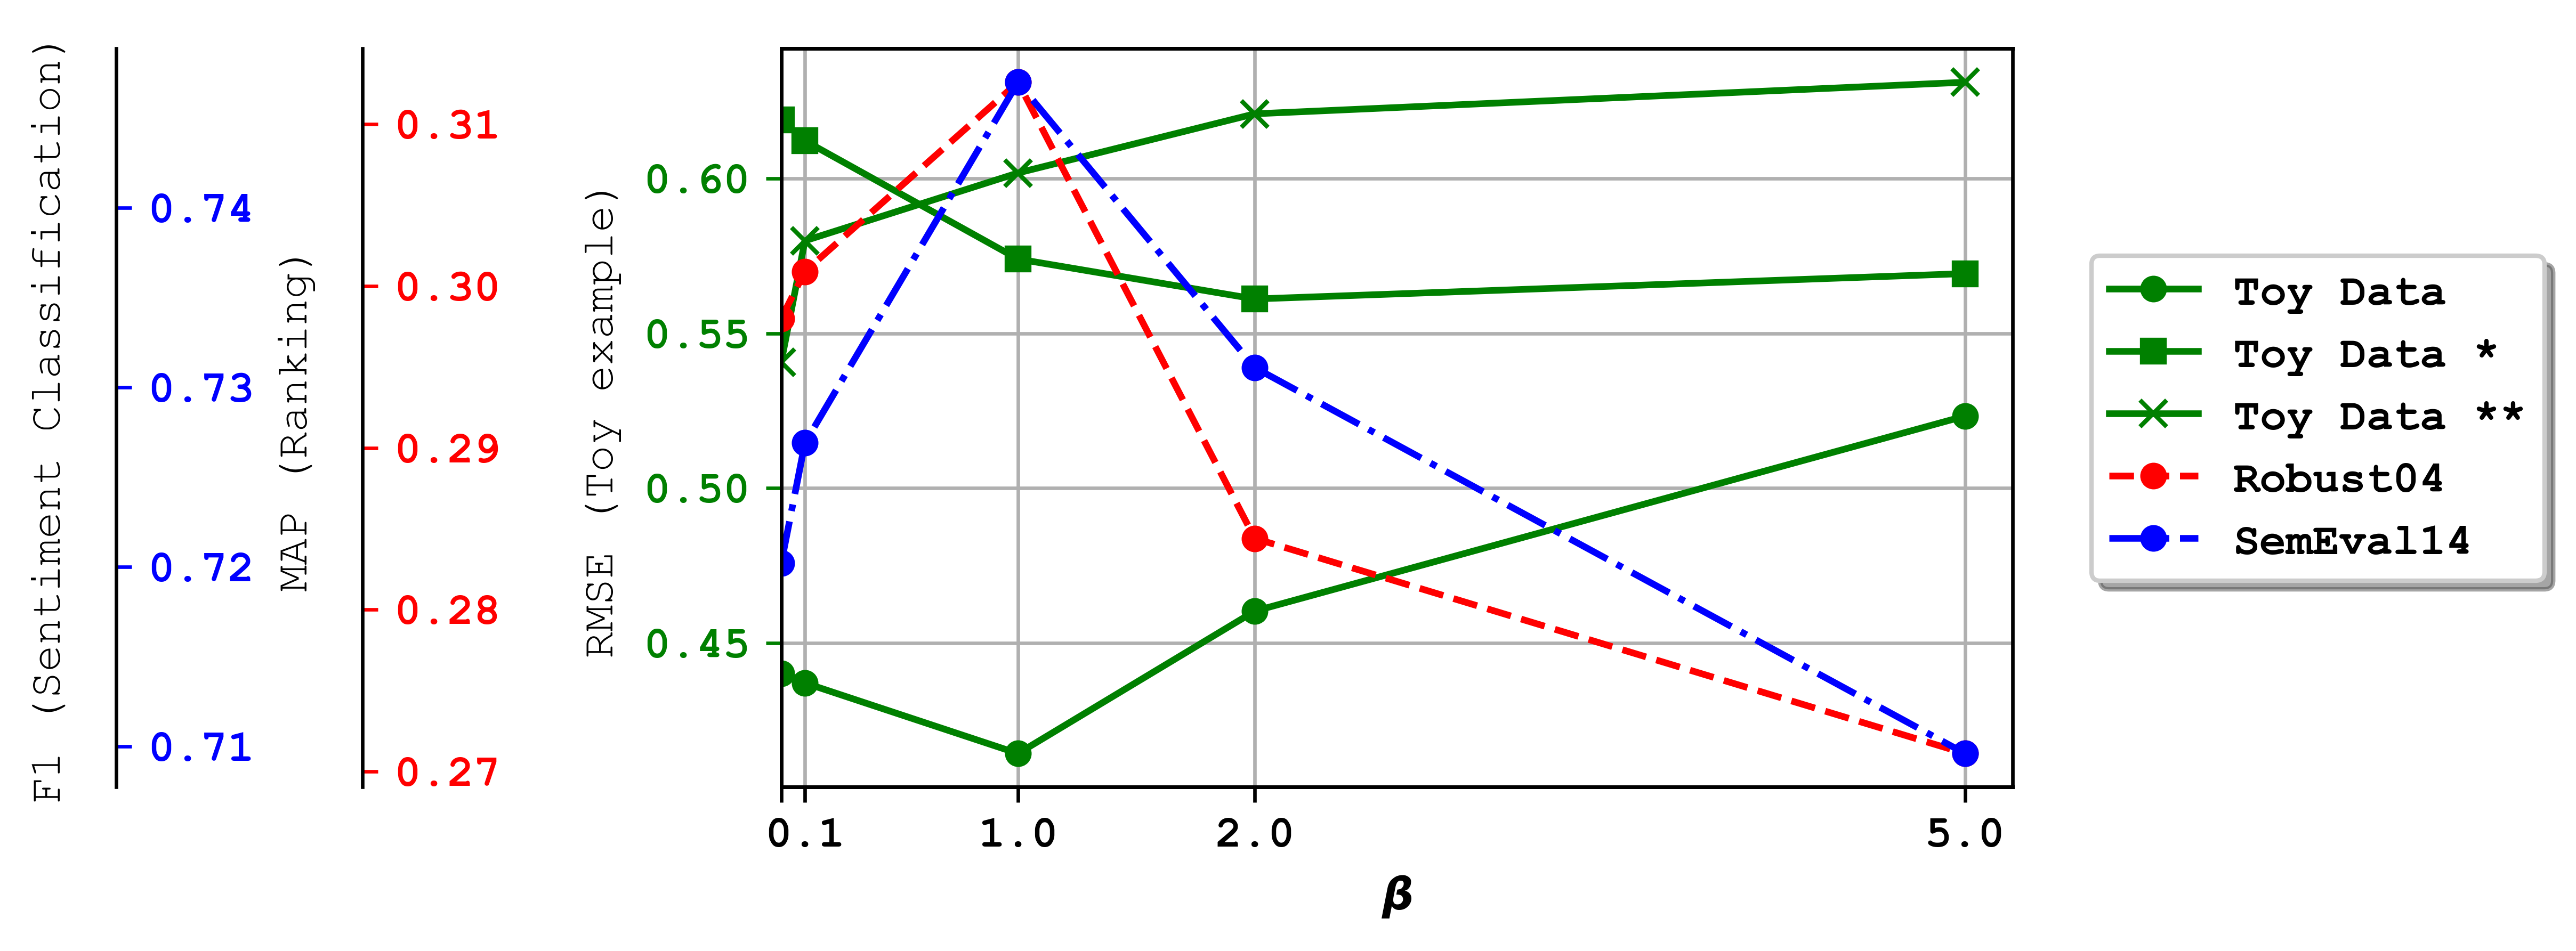
\includegraphics[width=0.7\textwidth]{03-part-02/chapter-05/figs_and_tables/plot_beta_fwl.png}
    \caption{Effect of different values for $\beta$.}
    \label{fig:beta}
\end{figure}

Figure~\ref{fig:beta} illustrates the performance on the ranking (on Robust04 dataset) and sentiment classification tasks (on SemEval14 dataset).  For both sentiment classification and ranking, $\beta=1$ gives the best results (higher scores are better).
%
We also experimented on the toy problem with different values of $\beta$ in three cases: 
1) having 10 observations from the true function (same setup as Section~\ref{sec:toy_exmpale}), marked as ``Toy Data'' in the plot, 
2) having only 5 observations from the true function, marked as ``Toy Data *'' in the plot, and 
3) having $f(x) = x + 1$ as the weak function, which is an extremely bad approximator of the true function, marked as ``Toy Data **'' in the plot.
%
For the ``Toy Data'' experiment, $\beta=1$ turned out to be optimal (here, lower scores are better). However, for ``Toy Data *'', where we have an extremely small number of observations from the true function, setting $\beta$ to a higher value acts as a regularizer by relying more on weak signals, and eventually leads to better generalization. 
On the other hand, for ``Toy Data **'', where the quality of the \wa is extremely low, lower values of $\beta$ put more focus on the true observations. Therefore, $\beta$ lets us control the bias-variance trade-off in these extreme cases.

We have also tested $\hat{c}_t = \eta_2(x_t) = \nicefrac{\beta}{\rm var}[\Sigma(x_t)]$.  The experiments showed that the exponential choice gives a better overall performance. 


\subsection{Sensitivity of the \fwl to the Quality of the Weak Annotator}
Our proposed setup in \fwl requires defining a so-called ``\wa'' to provide a source of weak supervision for unlabelled data. In Section~\ref{sec:bias-variance} we discussed the role of parameter $\beta$ for controlling the bias-variance trade-off by trying two weak annotators for the toy problem. 
Now, in this section, we study how the quality of the weak annotator may affect the performance of the \fwl, for the task of document ranking as a real-world problem.

To do so, besides BM25~\citep{Robertson:2009}, we use three other weak annotators: 
\begin{figure}[t]
    \centering
    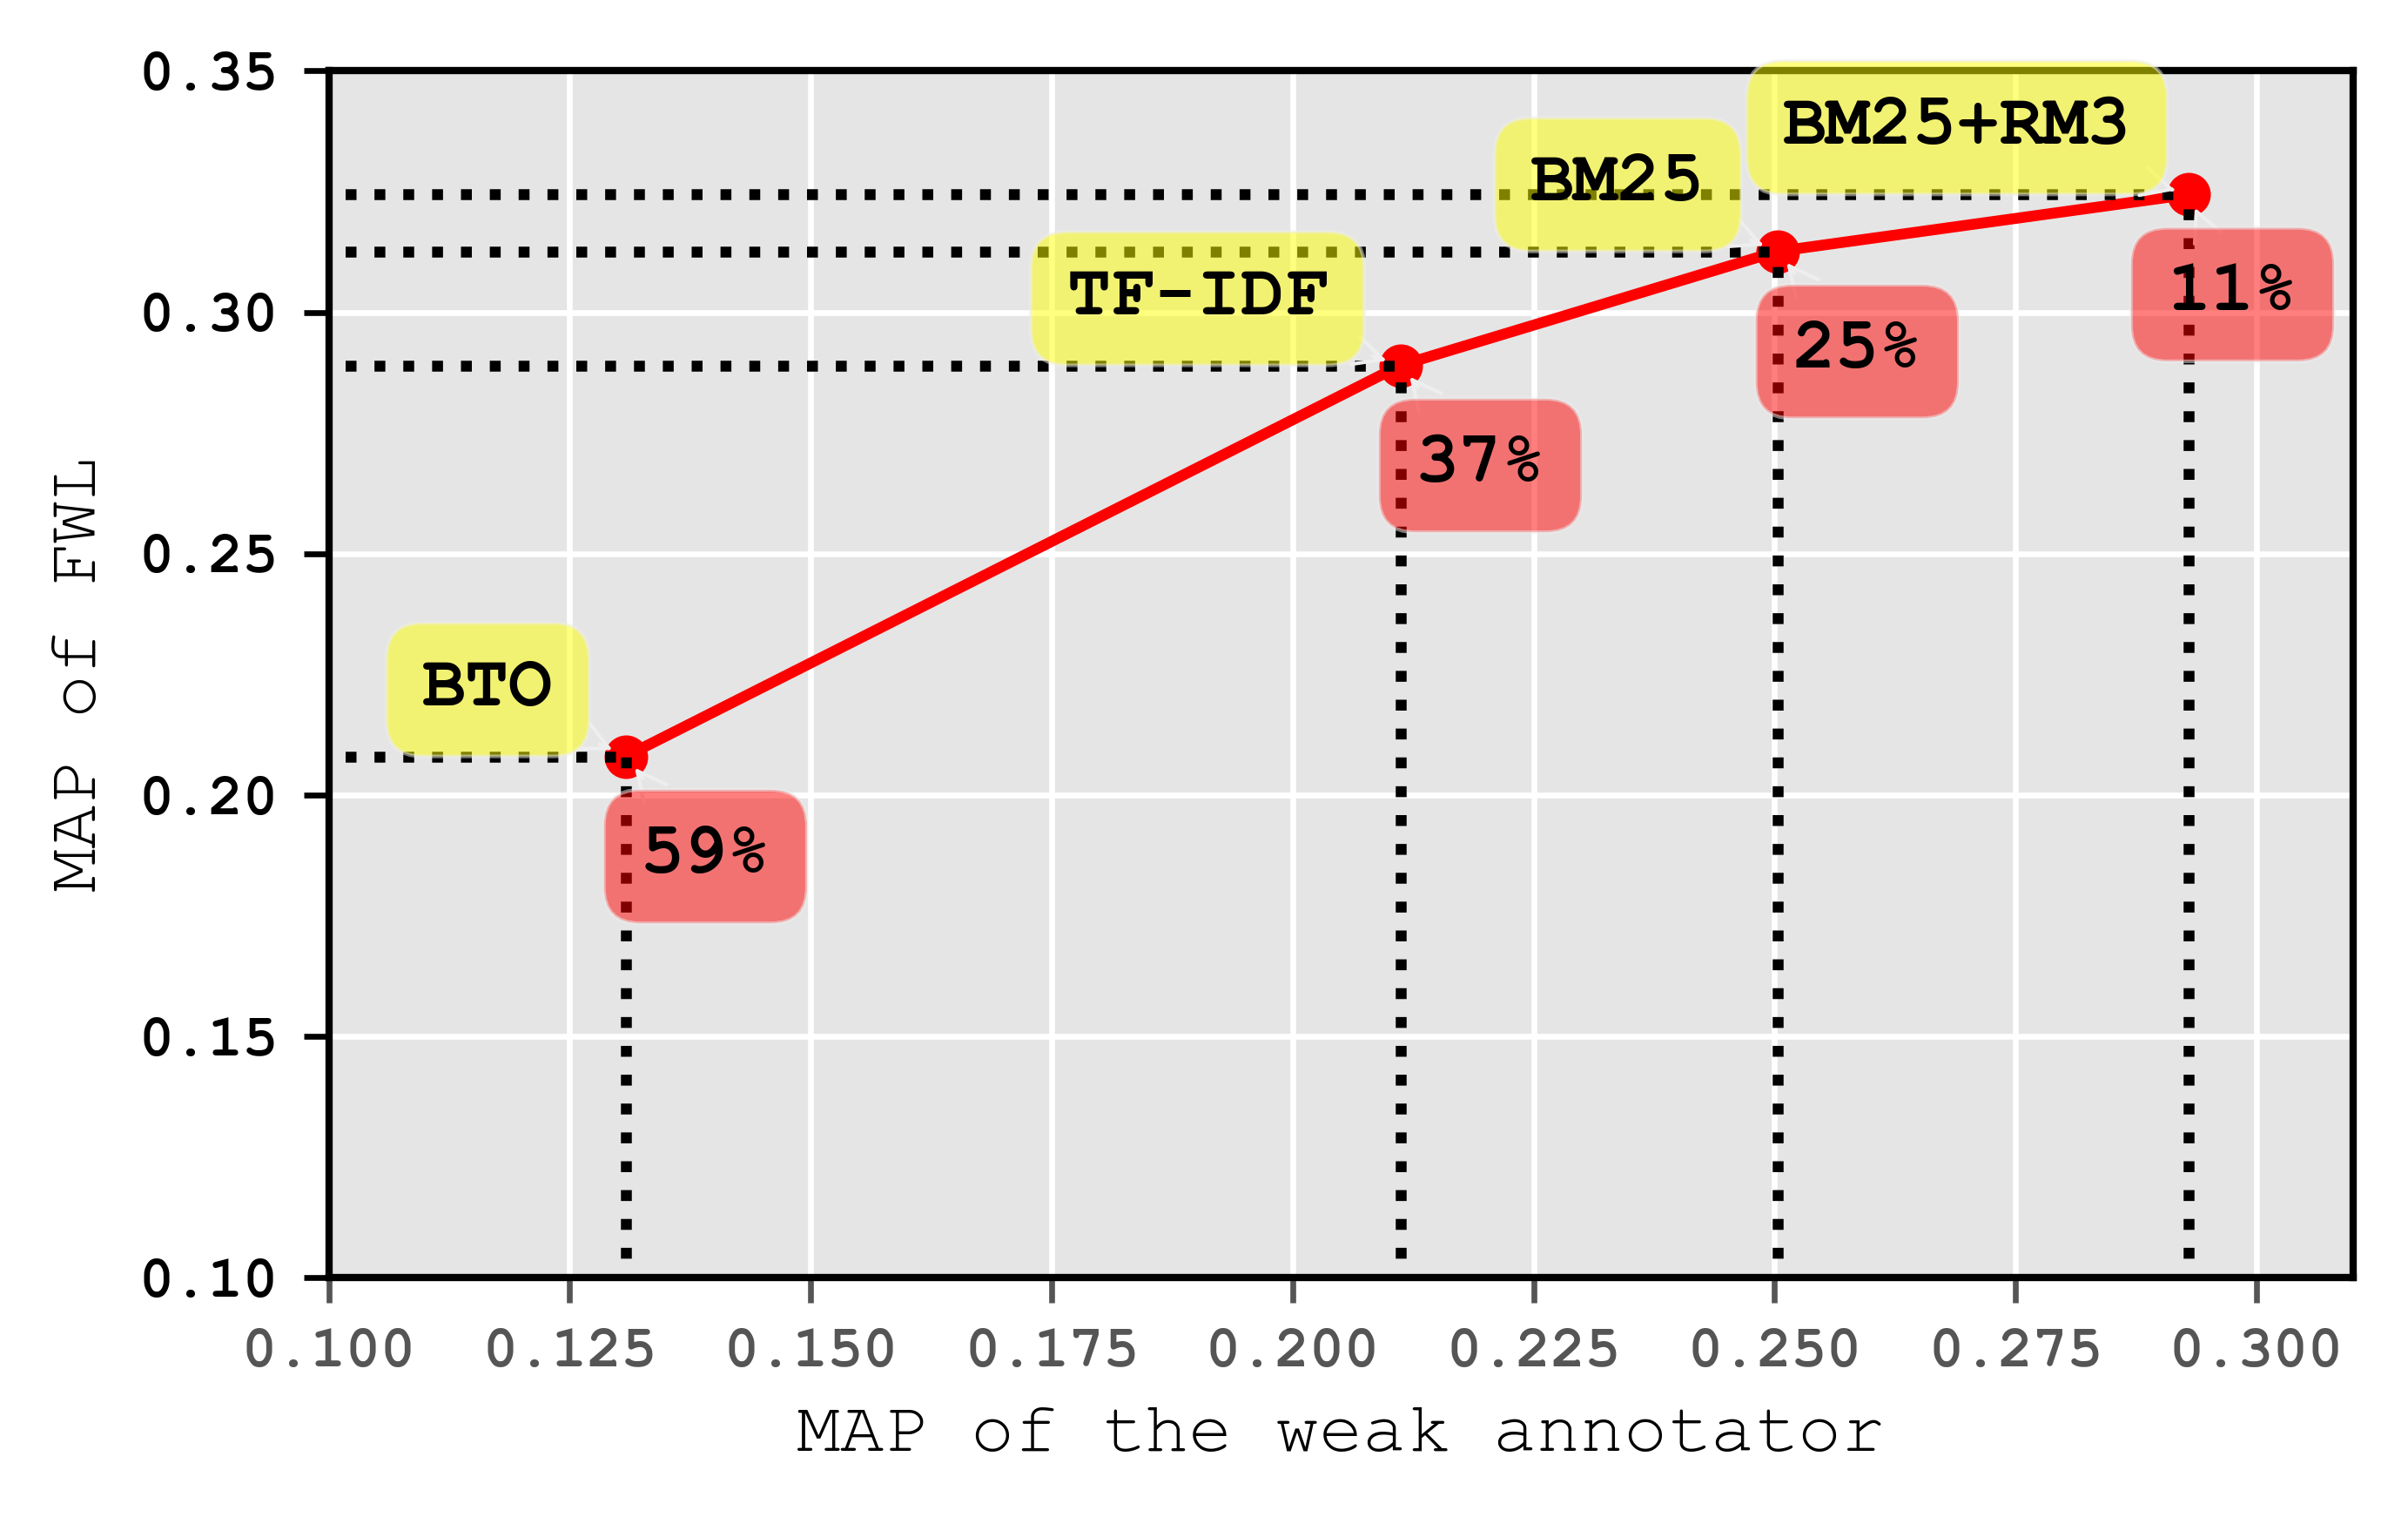
\includegraphics[width=0.7\textwidth]{03-part-02/chapter-05/figs_and_tables/plot_sensitivity_fwl.png}
    \caption{Performance of \fwl versus performance of the corespondence \wa in the document ranking task, on Robust04 dataset.}
    \label{fig:sensitivity}
\end{figure}
vector space model~\citep{salton1973specification} with binary term occurrence (BTO) weighting schema and vector
space model with TF-IDF weighting schema, which are both weaker than BM25, 
and BM25+RM3~\citep{Abdul-jaleel:2004} that uses RM3 as the pseudo-relevance feedback method on top of BM25, leading to better labels. 

Figure~\ref{fig:sensitivity} illustrates the performance of these four \was in terms of their mean average precision (MAP) on the test data, versus the performance of \fwl given the corresponding \wa. As it is expected, the performance of \fwl depends on the quality of the employed \wa.
The percentage of improvement of \fwl over its corresponding \wa on the test data is also presented in Figure~\ref{fig:sensitivity}. As can be seen, the better the performance of the \wa is, the less the improvement of the \fwl would be. 


\subsection{From Modifying the Learning Rate to Weighted Sampling}
\fwl provides confidence score based on the certainty associated with each generated label $\bar{y}_t$, given sample $x_t \in \mathcal{D}_{sw}$. We can translate the confidence score as how likely including $(x_t,\bar{y}_t)$ in the training set for the \std model improves the performance, and rather than using this score as the multiplicative factor in the learning rate, we can use it to bias sampling procedure of mini-batches so that the frequency of training samples are proportional to the confidence score of their labels.

We design an experiment to try \fwl with this setup (\fwlnospace$_s$), in which we keep the architectures of the \std and the \tch and the procedure of the  first two steps of the \fwl fixed, but we changed the step 3 as follows:

Given the soft dataset $\mathcal{D}_{sw}$, consisting of $x_t$, its label $\bar{y}_t$ and the associated confidence score generated by the \tch, we normalize the confidence scores over all training samples and set the normalized score of each sample as its probability to be sampled. 
Afterward, we train the \std model by mini-batches sampled from this set with respect to the probabilities associated with each sample, but without considering the original confidence scores in parameter updating.
This means the more confident the \tch is about the generated label for each sample, the more chance that sample has to be seen by the \std model.
\begin{figure}[t]
    \centering
    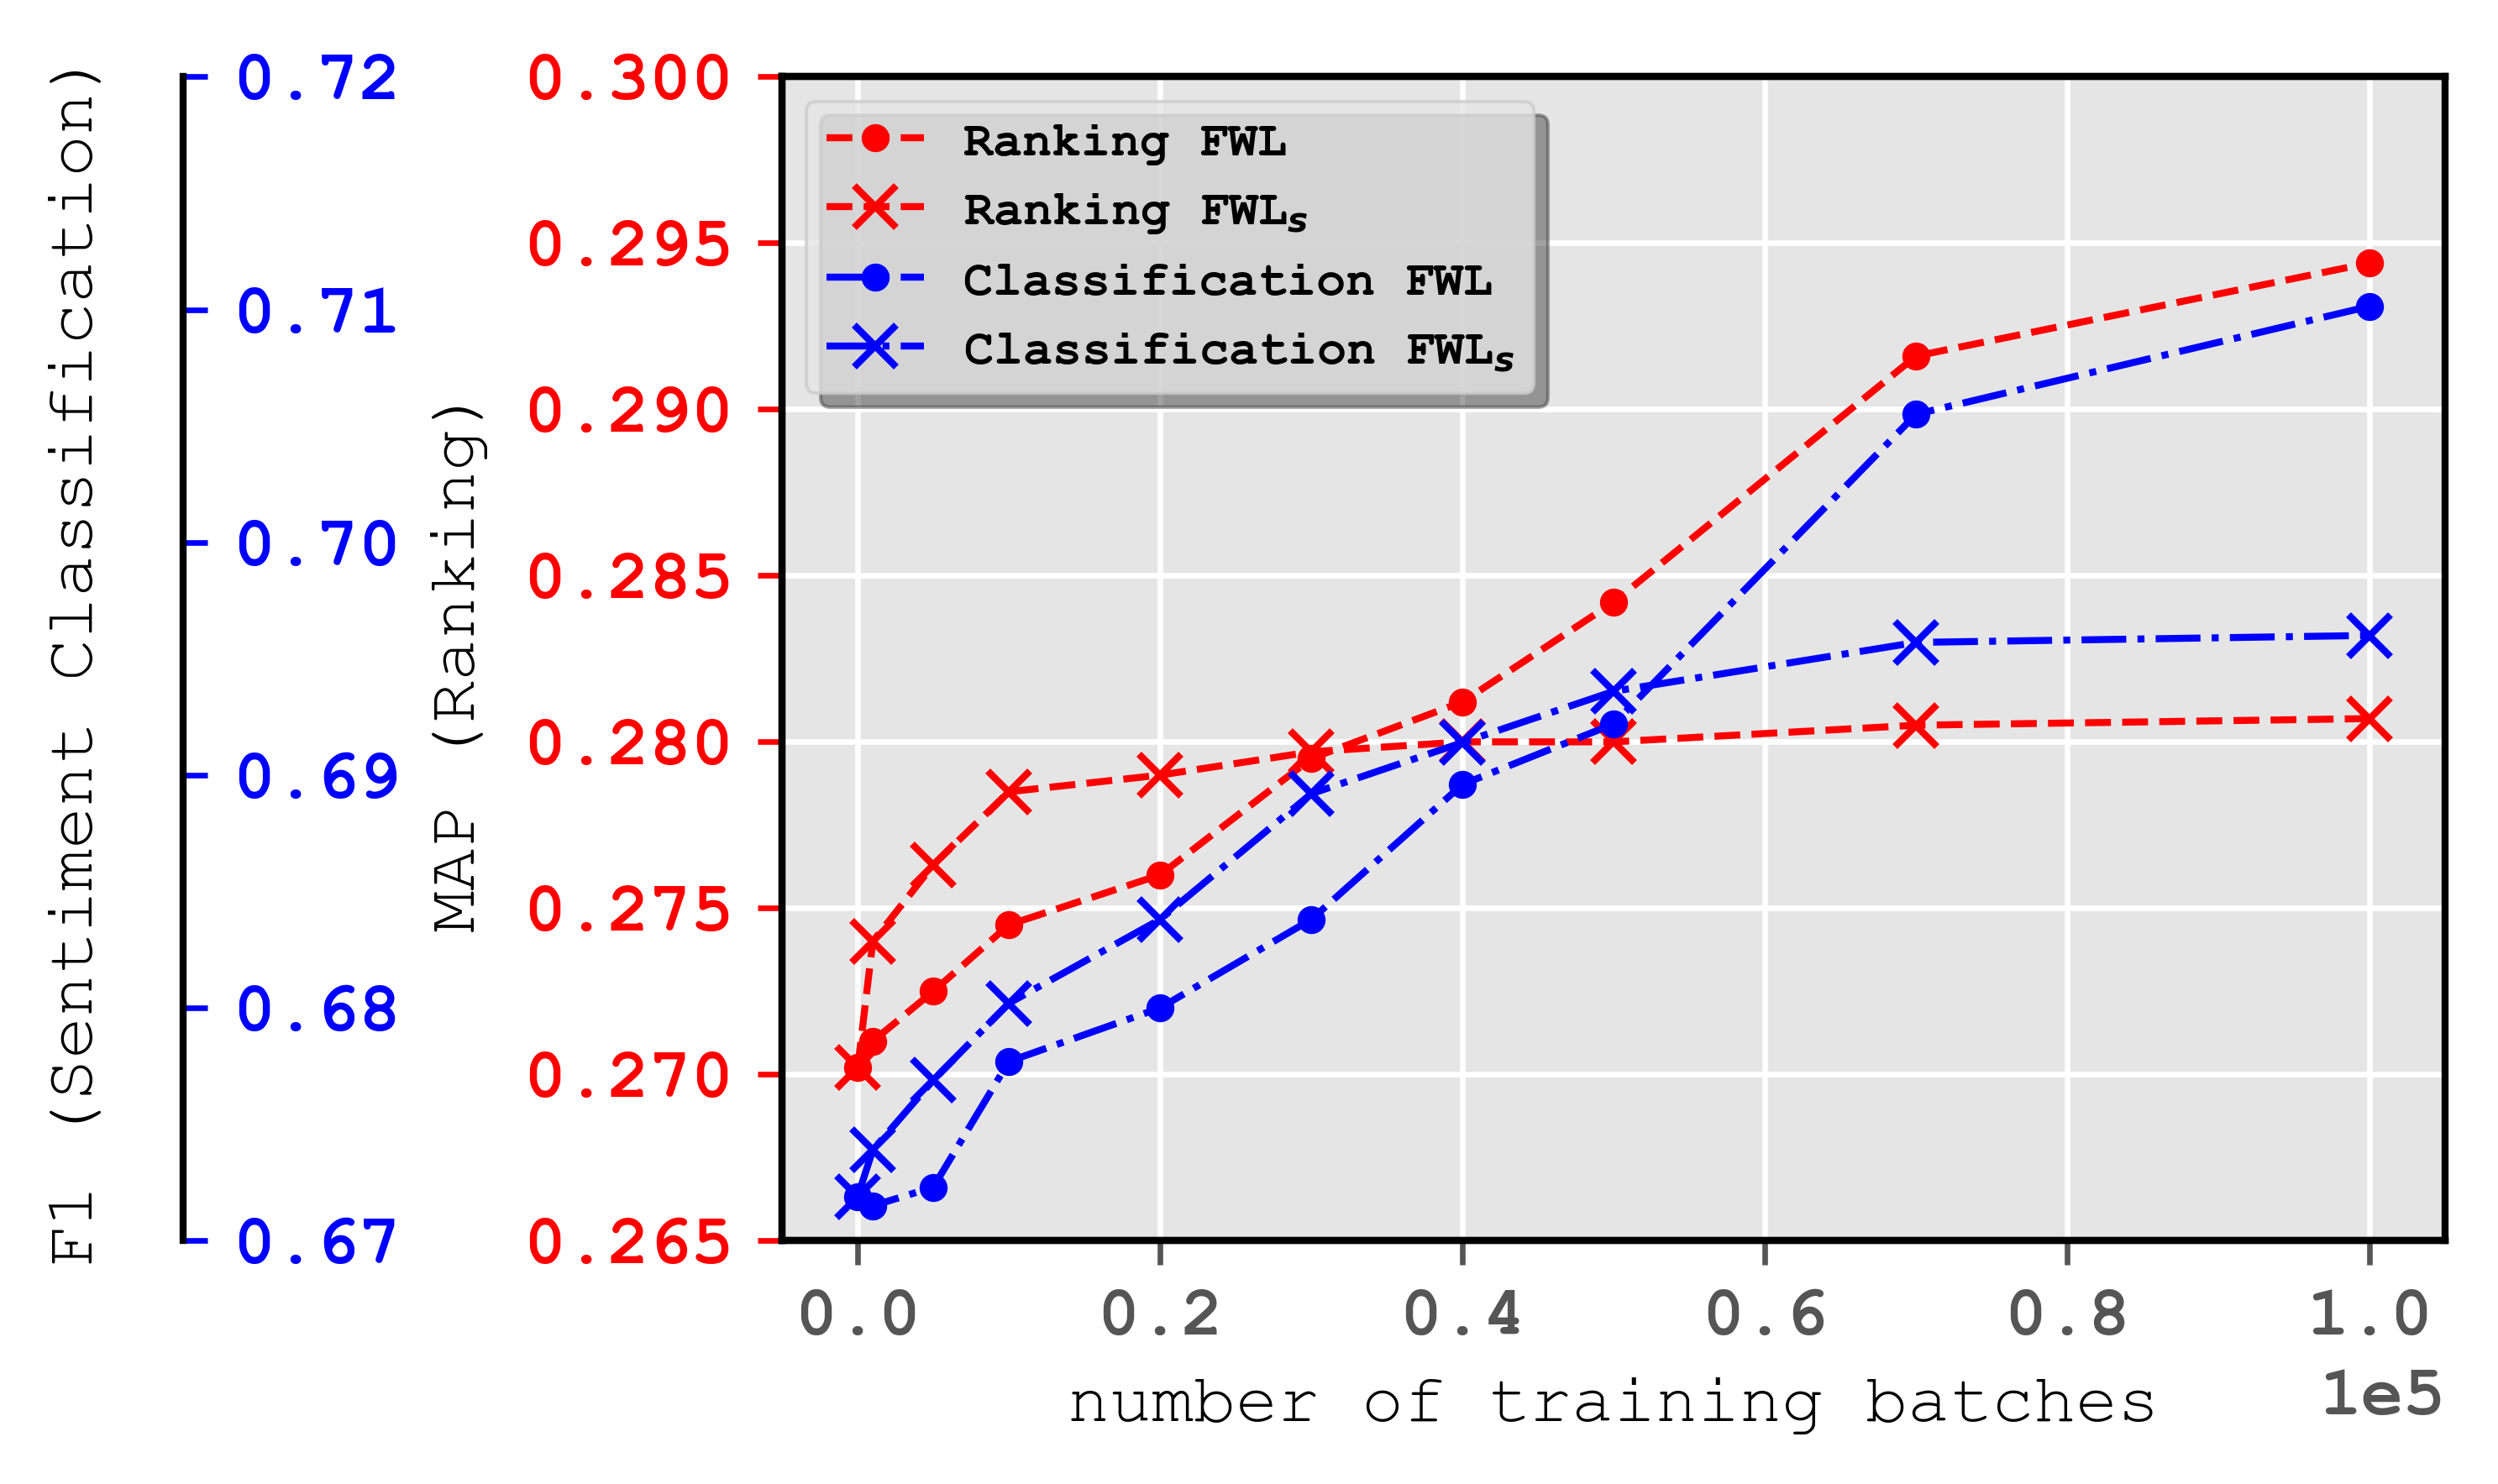
\includegraphics[width=0.7\textwidth]{03-part-02/chapter-05/figs_and_tables/plot_sampling_fwl.png}
    \caption{Performance of \fwl and \fwlnospace$_s$ with respect to different batch of data for the task of document ranking (Robust04 dataset) and sentiment classification (SemEval14 dataset).}
    \label{fig:sampling}
\end{figure}
Figure~\ref{fig:sampling} illustrates the performance of both \fwl and \fwlnospace$_s$ trained on different amount of data sampled from $\mathcal{D}_{sw}$, in the document ranking and sentiment classification tasks. 

As can be seen, compared to \fwl, the performance of \fwlnospace$_s$ increases rapidly in the beginning but it slows down afterward. 
We have looked into the sampling procedure and noticed that the confidence scores provided by the \tch form a rather skewed distribution and there is a strong bias in \fwlnospace$_s$ toward sampling from data points that are either in or closed to the points in $\mathcal{D}_{s}$, as $\mathcal{GP}$ has less uncertainty around these points and the confidence scores are high.
We observed that the performance of \fwlnospace$_s$ gets closer to the performance of \fwl after many epochs, while \fwl had already a log convergence.
%
The skewness of the confidence distribution makes \fwlnospace$_s$ to have a tendency for more exploitation than exploration, however, \fwl has more chance to explore the input space, while it controls the effect of updates on the parameters for samples based on their merit. 




\section{Related Work}
\label{sec:relatedwork}
In this section, we position the introduced \cws and \fwl approaches relative to related work.

\subsection{Learning from Imperfect Data}
Learning from imperfect labels has been thoroughly studied in the literature~\citep{Frenay:2014}.  The imperfect (weak) signal can come from non-expert crowd workers,  be the output of other models that are weaker (for instance with low accuracy or coverage), biased, or models trained on data from different related domains. 
%
Among these forms, in the distant supervision setup, a heuristic labeling rule~\citep{Deriu2016:SemEval,Severyn:2015:SemEval} or function~\citep{Dehghani:2017:SIGIR} which can be relying on a knowledge base~\citep{Mintz2009:distant,  min2013distant, Han:2016} is employed to devise noisy labels.  

Learning from weak data sometimes aims at encoding various forms of domain expertise or cheaper supervision from lay annotators. For instance, in the structured learning, the label space is pretty complex and obtaining a training set with strong labels is extremely expensive, hence this class of problems leads to a wide range of works on learning from weak labels~\citep{roth2017incidental}. 
%
Indirect supervision is considered as a form of learning from weak labels that is employed in particular in the structured learning, in which a companion binary task is defined for which obtaining training data is easier~\citep{Chang2010structured, Raghunathan:2016}. 

In the response-based supervision, the model receives feedback from interacting with an environment in a
task, and converts this feedback into a supervision
signal to update its parameters~\citep{roth2017incidental,clarke2010driving,riezler2014response}.
%
Constraint-based supervision is another form of weak supervision in which constraints that are represented as weak label distributions are taken as signals for updating the model parameters. For instance, physics-based constraints on the output~\citep{stewart2017label} or output constraints on execution of logical forms~\citep{clarke2010driving}.

In the proposed \cws and \fwl, we can employ these approaches as the weak annotator to provide imperfect labels for the unlabeled data, however, a small amount of data with strong labels is also needed, which put our model in the class of semi-supervised models. 

Some noise cleansing methods have been proposed to remove or correct mislabeled samples~\citep{Brodley:1999}.
There are some studies showing that weak or noisy labels can be leveraged by modifying the loss function~\citep{reed2014training, Patrini:2016, patrini2016loss, Vahdat:2017} or changing the update rule to avoid imperfections of the noisy data~\citep{malach2017decoupling, Dehghani:2017:nips_metalearn, Dehghani:2017avoiding}.  

One direction of research focuses on modeling the pattern of the noise or weakness in the labels. For instance, methods that use a generative model to correct weak labels such that a discriminative model can be trained more effectively~\citep{Ratner:2016,Rekatsinas:2017,Varma:2017}.
Furthermore, methods that aim at capturing the pattern of the noise by inserting an extra layer~\citep{goldberger2016training} or a separate module tries to infer better labels from noisy ones and use them to supervise the training of the network~\citep{Sukhbaatar:2014,Veit:2017, Dehghani:2017:nips_metalearn}. Our proposed \fwl can be categorized in this class as the \tch tries to infer better labels and provide certainty information which is incorporated as the update rule for the \std model.

\subsection{Semi-\:supervised Learning}
In the semi-supervised setup, some ideas were developed to utilize weakly or even unlabeled data. For instance, the idea of self(incremental)-training~\citep{Rosenberg:2005}, pseudo-labeling~\citep{Lee:2013,Hinton:2015}, and Co-training~\citep{Blum:1998} are introduced for augmenting the training set by unlabeled data with predicted labels.
Some research used the idea of self-supervised (or unsupervised) feature learning~\citep{noroozi2016unsupervised,dosovitskiy2016discriminative,donahue2016adversarial} to exploit different labelings that are freely available besides or within the data, and to use them as intrinsic signals to learn general-purpose features. These features, that are learned using a proxy task, are then used in a supervised task like object classification/detection or description matching.

As a common approach in semi-supervised learning, the unlabeled set can be used for learning the distribution of the data. In particular for neural networks, greedy layer-wise pre-training of weights using unlabeled data is followed by supervised fine-tuning~\citep{Hinton:2006,Deriu:2017,Severyn:2015:SemEval,Severyn:2015:SIGIR,Go:2009}. Other methods learn unsupervised encoding at multiple levels of the architecture jointly with a supervised signal~\citep{Ororbia:2015,Weston:2012}.


\subsection{Sentiment Classification and Document Ranking}
Sentiment classification is one of the key NLP tasks and SemEval provides standard benchmark datasets for this task~\citep{rosenthal:2015,Nakov:2016,rosenthal2017semeval}. There are many models proposed based on neural networks for sentiment classification task and in many datasets, the SOTA results are from convolutional-based models that learn multiple word vector representations~\citep{Kim:2014}. In our work, we adapt the CNN based architecture which is proposed to be trained with the help of weak (distance) supervising~\citep{Severyn:2015:SIGIR,Severyn:2015:SemEval,Deriu2016:SemEval} and has achieved SOTA results in some SemEval datasets~\citep{Deriu:2017}.
%
Document Ranking is also the core task of IR and some recent studies have applied neural networks on this task. Two main groups of models are those that learn representation for query and documents, independently,  and then use a matching function~\citep{Huang:2013,Mitra:2017,Shen:2014}, or models that try to capture interaction between query and document from the beginning~\citep{Lu:2013,Guo:2016,Dehghani:2017:SIGIR,Xiong:2017}. Here, we adapt a neural ranker with SOTA results that uses weak supervision~\citep{Dehghani:2017:SIGIR,dehghani:2018:ICLR}.



\section{Conclusion}
Training neural networks using large amounts of weakly annotated data is an attractive approach in scenarios where an adequate amount of data with true labels is not available, a situation which often arises in practice.

In this chapter, we introduced two semi-supervised learning approaches in the presence of weakly labeled data: Learning from Controlled Weak Supervision (\cws) and \fwlfulllc (\fwl).

\cws is a meta learning approach that unifies learning to estimate the confidence score of weak annotations and training neural networks to learn a target task with controlled weak supervision, i.e., using weak labels to updating the parameters but taking their estimated confidence scores into account. This helps to alleviate updates from instances with unreliable labels that may harm the performance.

\fwl is a student-teacher framework in which the student network is in charge of learning a target task given a vast amount of samples with weak labels associated with fertility scores that are generated by the teacher network. In \fwl, we pretrain the student network on weak data to learn an initial task-dependent data representation, which we pass to the teacher along with the strong data. The teacher then learns to predict the strong data, but crucially, \emph{based on the student's learned representation}. This then allows the teacher to generate new labeled training data from unlabeled data as well as fidelity scores for each sample in the data. Using samples in the new dataset, we update the parameters of the student network taking the fidelity scores into account to modulate the learning rate. 

We applied both \cws and \fwl to document ranking and sentiment classification, and empirically verified that they improve over state-of-the-art semi-supervised alternatives and speeds up the training process. We observed that the common approach of pre-training and fine-tuning is not as effective and found that explicitly modelling label quality is both possible and useful in this situation. 